\documentclass[12pt,a4paper]{report}

\usepackage[portuguese]{babel}
\usepackage{graphicx}
\usepackage{hyperref}
\usepackage{algorithm} 
\usepackage[noend]{algpseudocode}
\usepackage{caption}
\usepackage{bookmark}
\usepackage[nottoc,numbib]{tocbibind}
\usepackage{fancyhdr}
\usepackage{chngcntr}

\captionsetup[figure]{font=small}

\counterwithout{figure}{chapter}

\pagestyle{fancy}
\fancyhf{}
\lhead{VaccineRouter: transporte de vacinas entre centros de aplicação}
\cfoot{\thepage}

\DeclareCaptionFormat{algor}{
  \hrulefill\par\offinterlineskip\vskip1pt
    \textbf{#1#2}#3\offinterlineskip\hrulefill}
\DeclareCaptionStyle{algori}{singlelinecheck=off,format=algor,labelsep=space}
\captionsetup[algorithm]{style=algori}

\renewcommand\bibname{Referências}

\begin{document}


\begin{titlepage}
	\centering
	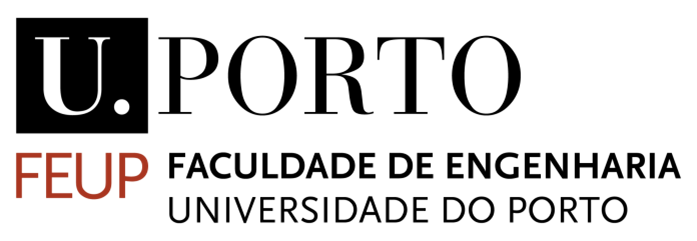
\includegraphics[width=0.6\textwidth]{../feup.png}\par\vspace{1cm}
	{\scshape Mestrado Integrado em Engenharia Informática e Computação \par}
	\vspace{1cm}
	{\scshape Concepção e Análise de Algoritmos \par}
	\vspace{1.5cm}
	{\huge VaccineRouter: transporte de vacinas entre centros de aplicação \par}
	\vspace{1cm}
	{\scshape Entrega 2}
	\vspace{4cm}
	
	{\scshape 2MIEIC05\_G2 \par}
	\vspace{0.5cm}

	{ Diogo Costa \href{mailto:up201906731@fe.up.pt}{up201906731@fe.up.pt} \par}
	{ Francisco Colino \href{mailto:up201905405@fe.up.pt}{up201905405@fe.up.pt} \par}
	{ Rui Alves \href{mailto:up201905853@fe.up.pt}{up201905853@fe.up.pt} \par}
	\vspace{2cm}
	

	{\large 21 maio 2021\par}
\end{titlepage}


\tableofcontents{}
\newpage
\listoffigures
\newpage

\chapter{Descrição do problema}
De forma a controlar a distribuição de vacinas contra a COVID-19, a aplicação VaccineRouter deve ser capaz de determinar os itinerários de distribuição de vacinas desde os centros de armazenamento até aos centros de aplicação. Como tal, pretende-se que estes itinerários não sejam demasiado extensos de forma a prevenir que o tempo de distribuição ultrapasse o tempo de conservação das vacinas.

	\section{Primeira Fase}
	Numa primeira instância, pretende-se que a aplicação seja capaz de definir um percurso para um único veículo, a sair de um único centro de armazenamento, não tendo como preocupação o tempo despendido para a distribuição das vacinas. \par
	Por outro lado, nesta primeira fase, não há preocupação acerca da capacidade dos veículos, de forma a garantir que apenas um veículo consiga distribuir vacinas para  todos os centros de aplicação. \par
	Para que tal distribuição seja possível, é necessário que existam caminhos que relacionem todos estes pontos de interesse, isto é, que existam ligações (estradas) que liguem o centro de distribuição com os vários centros de aplicação. Visto que estas ligações são representadas a partir de um grafo, este grafo terá de ser fortemente conexo (com ligações entre todos os vértices, no nosso caso sendo estes vértices os pontos de interesse), o que vai de acordo com a situação real à qual estamos a aplicar o problema. \par
	O objetivo desta fase trata-se, portanto, de encontrar a melhor rota, isto é, o percurso mais rápido, que uma carrinha tem de percorrer de forma a distribuir as vacinas em todos os centros de aplicação.

	\section{Segunda Fase}
	Numa segunda fase, é acrescentado ao problema o facto de termos vários centros de armazenamento, ou seja, teremos que distribuir os centros de aplicação pelos centros de armazenamento. Cada um dos centros de armazenamento terá, ainda, apenas um veículo com capacidade ilimitada. \par
	Este ponto irá levar a uma diminuição no tempo de distribuição das vacinas uma vez que teremos vários centros de armazenamento que, posteriormente, estarão mais perto de certos centros de aplicação. Este aumento de proximidade entre os vários centros (de aplicação e armazenamento) leva a que o tempo necessário para um dado veículo chegar a um centro de aplicação, saindo de um centro de armazenamento, seja menor do que o que tínhamos na primeira fase, onde uma carrinha tinha de distribuir as vacinas em todos os centros de aplicação.

	\section{Terceira Fase}
	Na terceira fase será adicionado o fator de tempo limite de distribuição e capacidade limitada das carrinhas. Tal como descrito anteriormente, as vacinas têm um tempo limitado de transporte, isto é, não podem estar muito tempo nas carrinhas que as irão distribuir (em transporte). Por outro lado, adicionando a restrição da capacidade limitada das carrinhas, poderão ocorrer casos em que mesmo que uma carrinha consiga percorrer os vários centros de aplicação no tempo pretendido, não tenha capacidade para levar as vacinas suficientes para os centros a que estava predestinada a distribuir. Isto leva, portanto, a que seja necessário adicionar mais veículos para fazer a sua distribuição a partir de um dado centro de armazenamento. \par
	O valor concreto de veículos por centro de armazenamento dependerá da performance de cada um destes, isto é, o tempo que demora a completar a distribuição. Para controlar esta condicionante, a solução passa por adicionar veículos que irão distribuir a partir desse centro, diminuindo, assim, o tempo de distribuição aos centros de aplicação associados a esse centro e, ainda, o número de veículos utilizados.


\chapter{Formalização do problema}

	\section{Dados de entrada}
	\begin{itemize}
		\item \( G_i = (V_i, E_i) \) - Grafo dirigido pesado, representado por:
		\begin{itemize}
			\item \( V_i \) - Vértices, onde \( V_i(i) \) representa o i-ésimo vértice, entre os quais se encontram os centros de distribuição e de aplicação, com:
			\begin{itemize}
				\item Id - identificador do vértice, único
				\item \( Adj \subseteq E \) - Arestas que partem do vértice
				\item Lat - latitude real do ponto no mapa
				\item Long - longitude real do ponto no mapa
			\end{itemize}

			\item \( E_i \) - Arestas, onde \( E_i(i) \) representa a i-ésima aresta, representando estradas da rede rodoviária, com:
			\begin{itemize}
				\item Id - identificador da aresta
				\item W - Peso da aresta, neste caso representando o tempo que demora a ser percorrida essa estrada
				\item \( Dest \in V_i \) - vértice ao qual a aresta liga o vértice inicial
			\end{itemize}
		\end{itemize}

		\item D - Conjunto dos Centros de Armazenamento, onde cada elemento \( D_i(i) \) é um vértice V que representa o i-ésimo Centro de Armazenamento caracterizado por:
		\begin{itemize}
			\item Nva - número de vacinas armazenadas
		\end{itemize}
		
		\item A - Conjunto dos Centros de Administração, onde cada elemento \( A_i(i) \) é um vértice V que representa o i-ésimo Centro de Administração caracterizado por:
		\begin{itemize}
			\item N - Número de vacinas que serão administradas nesse centro e, portanto, que têm de ser distribuídas para o mesmo
		\end{itemize}

		\item T - Tempo que as vacinas podem estar em transporte (nas carrinhas durante a distribuição desde os Centros de Armazenamento aos Centros de Administração) 

	\end{itemize}

		\subsection{Restrições dos dados de entrada}
		\begin{itemize}
			\item \( \forall E \in E_i, W(E) > 0 \), uma vez que \( w \) representa o tempo necessário para percorrer uma aresta
			\item \( \forall E \in Adj(V), Dest(E) \neq V \), uma vez que isso seria uma estrada de um ponto para ele próprio
			\item \( |D| > 0 \)
			\item \(|A| > 0 \land \forall a \in A, N(a) > 0 \), uma vez que caso seja 0, já não teremos de ir a esse centro de aplicação pois não se enquadra no nosso objetivo
			\item \(T > 0\)
			\item \(\sum_{d \in D} Nva(d) \geq \sum_{a \in A} N(a) \) (número de vacinas dos centros de armazenamento é maior ou igual ao número de vacinas pedido nos centros de administração)
		\end{itemize}


	\section{Dados de saída}
	\begin{itemize}
		\item \( G_f = (V_f, E_f) \) - Grafo dirigido pesado, sendo \( V_f \) e \( E_f \) os mesmos atributos que \( V_i \) e \( E_f \), à exceção de atributos que poderão ser acrescentados de forma a aplicar certos algoritmos.
		\item \(C_f\) - Sequência das carrinhas, onde \( C_f(i) \) representa a i-ésima carrinha, contendo o mesmo tipo de elementos que \( C_i \) à exceção de que estes terão mais quatro atributos:
		\begin{itemize}
			\item T - Tempo que a carrinha demorou a distribuir as vacinas
			\item P - Sequência de arestas E que irá percorrer de forma a distribuir as vacinas desde o Centro de Armazenamento, onde \( P_i \) representa a i-ésima aresta percorrida
			\item N - Número de vacinas que distribuiu
			\item C - Centro de armazenamento usado
		\end{itemize}
	\end{itemize}

	\subsection{Restrições dos dados de saída}
	\begin{itemize}
		\item \( \forall C \in C_f, N(C) > 0 \), isto é, todas as carrinhas que foram distribuir têm de distribuir pelo menos uma vacina
		\item \( |C_f| > 0 \)
		\item \( \forall c \in C_f, (T(c) > 0 \land T(c) \leq T)\)
		\item \( \forall c \in C_f \forall p \in P(c), p \in E \)
		\item \( |P| \leq |E| \)
		\item \( \forall c \in C_f \), número de vacinas por distribuir = 0, isto é, todas as carrinhas distribuem todas as vacinas que transportam
	\end{itemize}


	\section{Funções Objetivo}
	O principal objetivo deste problema é que as vacinas sejam todas distribuídas num dado tempo limite. Contudo, a melhor solução do mesmo passa por, após ter encontrado uma solução que entregue as vacinas dentro desse tempo limite, minimizar o número de carrinhas que as vão distribuir, de forma a tornar esta distribuição menos dispendiosa. \par
	Assim, primeiro pretende-se minimizar o tempo despendido pela carrinha que demora mais tempo (função \textit{f}), de forma que as vacinas não estejam em transporte mais do que o tempo limite (\textit{T}), e, secundariamente, minimizar o número de carrinhas que irão transportar as vacinas (função \textit{g}) aos centros de administração.

	\[ f = max([T(c)\, \forall c \in C_f]) < T\]
	\[ g = |C_f| \]



\chapter{Perspetivas de solução}
\label{perspetivas}
O problema proposto é semelhante ao \textit{Travelling Salesman Problem}, colocando agora mais opções para o percurso tomado, tal como a existência de várias carrinhas e de vários centros de armazenamento de onde estas saem. Este problema (\textit{TSP}) enquadra-se nos problemas \textit{NP-Hard} cujo objetivo é encontrar o menor caminho (em termos de tempo e custo) que passe por todos os pontos de interesse. \par
O facto de termos vários centros de distribuição leva a que este problema vá ao encontro da generalização do \textit{Vehicle routing problem}, ou seja, entramos no âmbito de \textit{Multi-depot vehicle routing problem}.

	\section{Acessibilidade}
	\label{perspetivas:acessibilidade}
	Acessibilidade diz respeito à possibilidade de, num dado grafo, aceder aos seus vértices a partir de outros. \par
	Para a analisar, poderemos usar algoritmos tal como o \textit{depth-first-search} (\textit{DFS}) ou \textit{breadth-first-search} (\textit{BFS}), que nos indicam os componentes conexos de um grafo.

		\subsection{\textit{Depth-First-Search algorithm}}
		\label{algo:dfs}
		Método de busca não-informada que avança através da expansão do primeiro nó encontrado no grafo avançando em profundidade até o objetivo ser encontrado ou já não existirem nós não visitados que sejam adjacentes; chegando a este ponto faz-se \textit{backtracking} e ao encontrar um nó com arestas cujos destinos não tenham sido ainda visitados o processo repete-se. Desta forma, este algoritmo tem uma complexidade temporal de \( O(|V| + |E|) \).

		\begin{center}
			\captionof{algorithm}{\textit{Depth-First-Search}}
			\begin{algorithmic}[1]
				\State $G = (V, E)$
				\newline
				\Function{DFS}{$G$}
					\For {$v \in V$}
						\State $ visited(v) \leftarrow false $
					\EndFor
					\For{$v \in V$}
						\If{$!visited(v)$}
								\State $DFS$-$VISIT(G, v)$
						\EndIf
					\EndFor
				\EndFunction
				\newline
				\Function{DFS-VISIT}{$G, v$}
					\State $ visited(v) \leftarrow true $
					\State $ pre$-$process(v) $
					\For{$w \in Adj(v)$}
						\If{$!visited(w)$}
							\State $DFS$-$VISIT(G, w)$
						\EndIf
					\EndFor
					\State $post$-$process(v)$
				\EndFunction
			\end{algorithmic}
		\end{center}

		\subsection{\textit{Breath-First-Search algorithm}}
		\label{algo:bfs}
		É também um método de busca não-informada que expande sequencialmente todos os vértices do grafo. Por cada vértice o algoritmo itera por todas as arestas deste e garante que nenhum vértice é visitado mais do que uma vez. Desta forma, este algoritmo tem uma complexidade temporal de \( O(|V| + |E|)\).

		\begin{center}
			\captionof{algorithm}{\textit{Breath-First-Search}} 
			\begin{algorithmic}[1]
				\State $G = (V, E)$
				\newline
				\Function{BFS}{$G$}
					\State choose s from G
					\State $ visit(s)$
					\State $insert(Q, s)$
					\While{$!empty(Q)$}
						\State $v \leftarrow extract(Q)$
						\For{$ e \in edges(v)$}
							\State $w \leftarrow destiny(e)$
							\If{$!visited(w)$}
								\State $visit(w)$
								\State $insert(Q, w)$
							\EndIf
						\EndFor
					\EndWhile
				\EndFunction
			\end{algorithmic}
		\end{center}
	

	\section{Conectividade forte}
	\label{perspetivas:conectividadeforte}
	De forma a podermos utilizar certos tipos de algoritmos, temos de, primeiro, averiguar a conectividade do grafo de entrada. Este, sendo um grafo que representa um mapa real, será um grafo esparso, pelo que teremos de confirmar se é possível navegar de um dado vértice para os outros, descartando os vértices que não são acessíveis. \par
	Para tal, poderemos usar o algoritmo de \textit{Kosaraju} ou o algoritmo de \textit{Tarjan}, cujo objetivo é encontrar as componentes fortemente conexas de um grafo dirigido, isto é, encontrar conjuntos de vértices onde todos os vértices desse conjunto são atingíveis a partir de qualquer outro vértice pertencente a esse mesmo conjunto.
	
		\subsection{\textit{Kosaraju algorithm}}
		\label{algo:kosaraju}
		O algoritmo de \textit{Kosaraju} é um algoritmo de complexidade linear cujo objetivo é encontrar componentes fortemente conexas de um grafo. O algoritmo foi sugerido por \textit{Sambasiva Kosaraju} em 1978, contudo apenas foi publicado independentemente em 1981 por \textit{Micha Sarir}. \cite{kosaraju} \par
		Este algoritmo consiste em fazer primeiro uma pesquisa em profundidade (\textit{DFS}), colocando os vértices visitados numa \textit{stack}, após ter sido feita a chamada recursiva \textit{DFS} aos seus vértices adjacentes; posteriormente, fazer o reverso do grafo, isto é, mudar a direção de todas as arestas do grafo; numa terceira fase, retirar elementos um a um da \textit{stack} (\textit{pop}) enquanto esta não estiver vazia. Sendo V o elemento retirado (\textit{popped}), aplicar a pesquisa em profundidade \textit{DFS} começando no vértice V; após este 2.º  \textit{DFS}, todos os vértices visitados irão formar uma componente fortemente conexa. \par
		Este algoritmo tem complexidade temporal \(O(|V| + |E|)\), pelo que se revela um bom algoritmo para este objetivo.

		\begin{center}
			\captionof{algorithm}{\textit{Kosaraju}} 
			\begin{algorithmic}[1]
				\State $G = (V, E)$
				\State $stack$ $stack$
				\State $vector$ $SCC$
				\State $int$ $component$
				\newline
				\Function{DFS1}{$G,s$}
					\State $visit(s)$
					\For{$v \in Adj(s)$}
						\If{$!visited(v)$}
							\State $DFS1(v)$
						\EndIf
					\EndFor
				\EndFunction
				\newline
				\Function{DFS2}{$G,component, s$}
					\State $visit(s) \leftarrow false$
					\State $SCC(component).push(s)$
					\For{$v \in Adj(s)$}
						\If{$!visited(v)$}
							\State $DFS2(G, component, s)$
						\EndIf
					\EndFor
				\EndFunction
				\newline
				\Function{Kosaraju}{$ $}
					\For{$v \in V$}
						\State $visit(s) \leftarrow false$
					\EndFor
					\For{$v \in V$}
						\State $DFS1(G,s)$
					\EndFor
					\State $G = getTranspose(G)$
					\For{$v \in V$}
						\State $visit(s) \leftarrow false$
					\EndFor
					\While{$!stack.empty$}
						\State $v \leftarrow stack.pop()$
						\If{$!visited(v)$}
							\State $DFS2(G, component, v)$
						\EndIf
						\State $component++$
					\EndWhile
					\State $return$ $SCC$
				\EndFunction
			\end{algorithmic}
		\end{center}


		\subsection{\textit{Tarjan's algorithm}}
		\label{algo:tarjan}
		O algoritmo de \textit{Tarjan} é outro algoritmo que poderemos usar para estudar a conectividade do grafo. Proposto em 1972 por \textit{Robert Tarjan} \cite{tarjan}, o algoritmo consiste em encontrar as componentes fortemente conexas a partir duma exploração em profundidade (\textit{DFS}) começando num vértice arbitrário. Atribuindo \textit{ids} e um \textit{low-link value} aos vértices utilizando uma \textit{stack}, o algoritmo agrupa os vértices que pertencem à mesma componente fortemente conexa na chamada recursiva da \textit{DFS}.

		\begin{center}
			\captionof{algorithm}{\textit{Tarjan}} 
			\begin{algorithmic}[1]
				\State $G = (V, E)$
				\State $stack$ $stack$
				\State $id \leftarrow 0$
				\State $sccCount \leftarrow 0$
				\newline
				\Function{DFS}{$G,s$}
					\State $stack.push(s)$
					\State $id(s) \leftarrow id++$
					\State $low(s) \leftarrow id(s)$
					\State $onstack(s) \leftarrow true$
					\For{$v \in Adj(s)$}
						\If{$id(v)=NULL$}
							\State $DFS(v)$
						\EndIf
						\If{$onstack(v)$}
							\State $low(s) \leftarrow min(low(s), low(v))$
						\EndIf
					\EndFor
					\If{$low(s)=id(s)$}
						\While{$(v \leftarrow stack.pop()) \neq s$}
							\State $onstack(v) \leftarrow false$
							\State $low(v) \leftarrow id(s)$
							\State $SCC(v) \leftarrow s$
						\EndWhile
						\State $SCC(s) \leftarrow s$
					\EndIf
				\EndFunction
				\newline
				\Function{Tarjan}{$G$}
				\For{$u \in V$}
					\State $id(u) \leftarrow NULL$
					\State $SCC(u) \leftarrow NULL$
				\EndFor
				\For{$u \in V$}
					\If{$id(u) = NULL$}
						\State $DFS(G,u)$
					\EndIf
				\EndFor
				\State return SCC
				\EndFunction
			\end{algorithmic}
		\end{center}


	\section{Caminho mais curto}
	\label{perspetivas:caminhomaiscurto}
	Para resolvermos o problema em questão, teremos, também, de calcular o caminho mais curto entre dois vértices do grafo, de forma a, posteriormente, conseguirmos conectar os vários centros de administração ao centro de distribuição a si referenciado. \par
	Desta forma, pretende-se, com os seguintes algoritmos, determinar o caminho mais curto entre um vértice de origem e um vértice de destino.

		\subsection{\textit{Dijkstra algorithm}}
		\label{algo:dijkstra}
		O algoritmo de \textit{Dijkstra} é talvez o mais conhecido algoritmo para calcular o caminho mais curto, sendo que parte do pressuposto que não há arestas negativas. \par
		Primeiramente, todos os vértices são marcados com distância infinita até ao vértice de origem, exceto o próprio, que é marcado com distância 0. Após isso, fazem-se sucessivas visitas aos vértices adjacentes \( V_{adj} \)  do vértice \(V_p\) com distância menor e atualiza-se a distância mínima a eles passando pelo vértice considerado \(V_p\) e a aresta que os conecta. Assim, este algoritmo, utilizando uma fila de prioridade de mínimos, tem uma complexidade temporal \(O((|V|+|E|)\cdot log|V|)\), apesar de poder ser melhorada para \(O(|V|\cdot log|V|)\) utilizando \textit{Fibonacci Heaps}.

		\begin{center}
			\captionof{algorithm}{\textit{Dijkstra}}
			\begin{algorithmic}[1]
				\State $G = (V, E)$
				\State $s \in V$
				\newline
				\Function{Dijkstra}{$G,s$}\Comment{using a priority queue}
				\For{$v \in V$}
					\State $dist(v) \leftarrow INF$
					\State $path(v) \leftarrow NULL$
				\EndFor
				\State $dist(s) \leftarrow 0$
				\State $Q \leftarrow V$\Comment{Q is a min-priority queue of dist}
				\While{$|Q| > 0$}
					\State $v \leftarrow Q.extract\_min()$
					\For{$u \in Adj(v)$}
						\State $dist\_temp \leftarrow dist(v) + weight(v,u)$
						\If{$dist\_temp < dist(u)$}
							\State $dist(u) \leftarrow dist\_temp$
							\State $path(u) \leftarrow v$
							\State $Q.decrease\_key(u,dist(u))$
						\EndIf
					\EndFor
				\EndWhile
				\State return G
				\EndFunction
			\end{algorithmic}
		\end{center}


		\subsection{\textit{A* algorithm}}
		\label{algo:astar}
		O algoritmo \textit{A*} \cite{astar} é também um algoritmo bastante conhecido de caminho mais curto, sendo este uma extensão do algoritmo de \textit{Dijkstra} usando métodos heurísticos. Trata-se de uma pesquisa informada que averigua primeiro os caminhos mais promissores, fazendo uso de uma função heurística \textit{h}. \par
		Em termos simples, enquanto que o algoritmo de \textit{Dijkstra} seleciona o próximo vértice a averiguar pelo mínimo de distância até ele, o algoritmo \textit{A*} escolhe o vértice v que minimiza \(f(v) = dist(v) + h(v)\) sendo \textit{h(v)} a função heurística. Para \textit{h(v)} pode ser usado, por exemplo, a distância euclidiana de v até ao vértice final. Confirma-se, ainda, que o algoritmo de \textit{Dijkstra} é um caso particular do algoritmo \textit{A*} em que \( h(v) = 0 \). Desta forma, a complexidade do algoritmo \textit{A*} é semelhante à complexidade do algoritmo de \textit{Dijkstra} apenas com uma pequena ponderação dependendo da função \textit{h(v)} usada.

		\begin{center}
			\captionof{algorithm}{\textit{A*}}
			\begin{algorithmic}[1]
				\State $G = (V, E)$
				\State $s \in V$
				\newline
				\Function{Astar}{$G,s$}\Comment{using a priority queue}
				\For{$v \in V$}
					\State $dist(v) \leftarrow INF$
					\State $hdist(v) \leftarrow INF$
					\State $path(v) \leftarrow NULL$
				\EndFor
				\State $dist(s) \leftarrow 0$
				\State $hdist(s) \leftarrow h(s)$
				\State $Q \leftarrow V$\Comment{Q is a min-priority queue of hdist}
				\While{$|Q| > 0$}
					\State $v \leftarrow Q.extract\_min()$
					\For{$u \in Adj(v)$}
						\State $dist\_temp \leftarrow dist(v) + weight(v,u)$
						\If{$dist\_temp < dist(u)$}
							\State $dist(u) \leftarrow dist\_temp$
							\State $path(u) \leftarrow v$
							\State $Q.decrease\_key(u,dist(u)+h(u))$
						\EndIf
					\EndFor
				\EndWhile
				\State return G
				\EndFunction
			\end{algorithmic}
		\end{center}


		\subsection{\textit{Floyd-Warshall algorithm}}
		\label{algo:floydwarshall}
		O algoritmo de \textit{Floyd-Warshall}, publicado independentemente por \textit{R. W. Floyd} e \textit{S. Warshall} em 1962 difere nos mencionados anteriormente no facto de encontrar o caminho mais curto entre todos os vértices numa única execução. O algoritmo mantém uma matriz de distâncias que vai sendo atualizada à medida que vão sendo considerados diferentes vértices intermédios. \par
		Este algoritmo tem uma complexidade temporal de \( O(|V|^3)\) e espacial de \( O(|V|^2)\).

		\begin{center}
			\captionof{algorithm}{\textit{Floyd-Warshall}}
			\begin{algorithmic}[1]
				\State $G = (V, E)$
				\newline
				\Function{FloydWarshall}{$G$}
				\State $distM \leftarrow matrix(|V|, |V|)$
				\State $fill(distM, INF)$
				\For{$e \in E$}
					\State $distM[orig(e), dest(e)] \leftarrow dist(e)$
				\EndFor
				\For{$i=1$ to $|V|$}
					\State $distM[i,i] \leftarrow 0$
				\EndFor
				\For{$k=1$ to $|V|$}
					\For{$i=1$ to $|V|$}
						\For{$j=1$ to $|V|$}
							\If{$distM[i, j] > distM[i, k] + distM[k, j] $}
								\State $distM[i,j] \leftarrow distM[i, k] + distM[k, j]$
							\EndIf
						\EndFor
					\EndFor
				\EndFor
				\State $return$ $distM$
				\EndFunction
			\end{algorithmic}
		\end{center}
	
	
	\section{\textit{Travelling Salesman Problem}}
	\label{perspetivas:tsp}
	Este é o problema de encontrar o caminho mais curto e eficiente para o Salesman de forma a passar em todos os seus pontos de interesse. Existem diferentes métodos usados para resolver este problema, entre eles:
	\begin{itemize}
		\item \textit{Brute-Force}
		\item \textit{Branch and Bound}
		\item \textit{Nearest Neighbor}
	\end{itemize}

		\subsection{\textit{Bellman-Held-Karp algorithm}}
		\label{algo:bellmanheldkarp}
		Uma possível solução exata para este problema é a utilização do algoritmo de \textit{Bellman-Held-Karp}. \par
		Este algoritmo foi proposto independentemente em 1962 por \textit{Richard Bellman}, \textit{Michael Held} e por \textit{Richard Karp} e consiste na utilização de programação dinâmica, resolvendo o exercício geral e mais complexo a partir da resolução de subproblemas do mesmo, isto é, a solução do problema pode ser obtida a partir das soluções dos seus subproblemas. \par
		Este algoritmo oferece-nos uma complexidade temporal relativamente boa (inferior à complexidade da abordagem \textit{brute-force} que é de ordem fatorial) de \( O(|V|^2 \cdot 2^{|V|})\) mas, por outro lado, tem uma complexidade espacial \( O(|V| \cdot 2^{|V|})\), ambas no pior caso. \cite{bellmanheldkarp} \par
		Assim sendo, e uma vez que os grafos com os quais vamos lidar serão relativamente grandes, não vai ser útil um algoritmo de ordem exponencial e como tal, não será usado na implementação. Ainda assim, achamos por bem fazer referência a ele dado que se trata de um algoritmo exato.

		\begin{center}
			\captionof{algorithm}{\textit{Bellman-Held-Karp}}
			\begin{algorithmic}[1]
				\State $G = (V, E)$
				\newline
				\Function{BellmanHeldKarp}{$G$}
				\State $s \leftarrow inicial$ $vertex$
				\For{$v \in V$}
					\State $OPT[\{v\}, v] \leftarrow weight(s,v)$
				\EndFor
				\For{$i=2$ to $|V|$}
					\For{$S \subseteq V-s$ with $|S| = i$}
						\For{$v \in S$}
							\State $ OPT[S,v] \leftarrow min\{OPT[S - v, u] + weight(u, v)$ | $u \in S - v \})$
						\EndFor
					\EndFor
				\EndFor
				\State $return$ $min\{ OPT[V - s, v] + weight(v, s)$ | $v \in V - s \} $
				\EndFunction
			\end{algorithmic}
		\end{center}



		\subsection{\textit{Nearest neighbor (NN) algorithm}}
		\label{algo:nn}
		O \textit{Nearest neighbor (NN) algorithm} \cite{nearestneighbor} foi um dos primeiros métodos usados para resolver o \textit{TSP}. Passa por escolher um ponto onde começar e escolhe o vértice adjacente a este cuja aresta que os ligue tenha menor peso e ainda não tenha sido visitado. \par
		No caso em concreto deste trabalho, em vez de escolher o vértice adjacente mais próximo, é escolhido o ponto de interesse mais próximo, que pode ser, por exemplo, obtido usando o algoritmo \textit{A*} com origem no vértice atual. Outra possibilidade será a de condensar o grafo de input para um outro, cujos únicos vértices são os pontos de interesse (\textit{POI}), ou seja, os centros de armazenamento e os centros de aplicação. \par
		O resultado é a ordem pela qual os vértices foram visitados. \par
		Este sendo um algoritmo que procura obter a solução a partir da melhor escolha em cada momento (indo ao vértice mais próximo), revela-se um algoritmo ganancioso. Ainda que o problema não possua subestrutura ótima e, como tal, o algoritmo não garanta a solução ótima, o \textit{NN} apresenta bons resultados. \par
		Este algoritmo tem, no pior caso, uma complexidade temporal de \(O(|V|^2) \) e espacial de \( O(|V|)\).

		\begin{center}
			\captionof{algorithm}{\textit{Nearest neighbor}}
			\begin{algorithmic}[1]
				\State $G = (V, E)$
				\newline
				\Function{NN}{$G$}
				\For{$v \in V$}
					\State $visited(v) \leftarrow false$
				\EndFor

				\State $v \leftarrow select(V, 0)$
				\State $visited(v) \leftarrow true$

				\State $S \leftarrow \emptyset$
				\State $ insert(S, v) $

				\State $count \leftarrow 0$
				\While{$count < size(V)$}
					\State $Q \leftarrow \emptyset$

					\For{$e \in edges(v)$}
						\State $insert (Q, (destiny(e), distance))$
					\EndFor

					\While{$size(Q) > 0$}
						\State $w \leftarrow extractMin(Q)$
						\If{$!visited(w)$}
							\State $increment(count)$
							\State $visited(w) \leftarrow true$
							\State $v \leftarrow w$
							\State $insert(S,v)$
							\State $break$
						\EndIf
					\EndWhile

				\EndWhile
				\State $return$ $G$
				\EndFunction
			\end{algorithmic}
		\end{center}


	
	\section{\textit{Vehicle routing Problem}}
	\textit{Vehicle routing problem} pode ser considerado um \textit{Travelling Salesman Problem} (\textit{TSP}) com vários \textit{Salesman}, sendo os \textit{Salesman} os veículos e como o tradicional \textit{TSP} tem diversos destinos pelos quais tem de passar. O objetivo é distribuir pelos diversos veículos os destinos de forma que todos sejam visitados, sendo esta distribuição otimizada de forma que o tempo total de distribuição (de todos os percursos aquele que demorar mais tempo) seja o menor possível. \par
	Para fazer esta distribuição de destinos a veículos existem diversos métodos, entre eles os heurísticos. \par
	Com a distribuição feita para cada instância de veículo e respetivos destinos temos um subproblema de \textit{Travelling Salesman}. Resolve-se este problema de forma a obter o caminho mais pequeno possível.
	
	
	\section{\textit{Multi-depot Vehicle routing Problem}}
	\label{perpetivas:mdvrp}
	\textit{Multi-depot vehicle routing problem} é uma generalização do \textit{Vehicle routing problem} no qual, para além de haver vários veículos, existem também vários armazéns, sendo este o problema com que estamos a lidar para fazer a distribuição das vacinas. \par
	A abordagem que seguiremos será fazer \textit{clustering} dos centros de aplicação pelos centros de armazenamento de forma a subdividir este problema mais complexo em múltiplos subproblemas do \textit{Vehicle Routing problem}. \par
	
		\subsection{\textit{Multi-source Dijkstra algorithm}}
		\label{algo:msdijkstra}
		O método usado para fazer os clusters será fazer múltiplas pesquisas em largura “simultaneamente” a partir de todos os centros de armazenamento até todos os centros de distribuição estarem no \textit{cluster} de um centro de armazenamento. Este método acaba por ser uma variante do algoritmo de \textit{Dijkstra} com múltiplas origens.


		\begin{center}
			\captionof{algorithm}{\textit{Multi-source Dijkstra}}
			\begin{algorithmic}[1]
				\State $ G = (V, E) $
				\State $ S \subseteq V $
				\newline
				\Function{MultiDijkstra}{$G,S$}
				\For{$v \in V$}
					\State $dist(v) \leftarrow INF$
					\State $path(v) \leftarrow NULL$
				\EndFor
				\For{$s \in S$}
					\State $dist(s) \leftarrow 0$
				\EndFor
				\State $Q \leftarrow V$\Comment{Q is a min-priority queue of dist}
				\While{$|Q| > 0$}
					\State $v \leftarrow Q.extract\_min()$
					\For{$u \in Adj(v)$}
						\State $dist\_temp \leftarrow dist(v) + weight(v,u)$
						\If{$dist\_temp < dist(u)$}
							\State $dist(u) \leftarrow dist\_temp$
							\State $path(u) \leftarrow v$
							\State $Q.decrease\_key(u,dist(u))$
						\EndIf
					\EndFor
				\EndWhile
				\State return G
				\EndFunction
			\end{algorithmic}
		\end{center}


		Neste pseudocódigo, por questões de simplicidade, o algoritmo só termina quando todos os vértices forem processados, sendo que o \textit{cluster} de um dado centro de distribuição \textit{CD} pode ser obtido a partir de \textit{path(CD)}. Para além disso, no programa terá que se ter em conta a quantidade de vacinas que cada centro de armazenamento tem, dado que, não adianta adicionar um centro de administração ao \textit{cluster} do centro de armazenamento mais próximo dele se este já não tiver vacinas suficientes.
	

\chapter{Casos de utilização}
O nosso programa deve permitir as seguintes funcionalidades:
	\begin{itemize}
		\item Fazer a distribuição dos centros de administração pelos centros de armazenamento (\textit{clustering}).
		\item Definir o número de veículos necessários para a distribuição de vacinas, as suas rotas e tempo utilizado em viagem por cada um, respeitando as restrições do problema.
		\item Possivelmente, fazer uso de uma ferramenta externa de visualização de grafos de forma a observar a rota de cada veículo.
		\item Obter as componentes fortemente conexas do grafo de entrada.
		\item Obter, caso existam, os centros de administração inacessíveis.
	\end{itemize}


\chapter{Funcionalidades e cenários implementados}
\label{func}
O nosso programa vai acompanhado dos seguintes mapas: Porto, Espinho, Penafiel e correspondentes componentes
fortemente conexas de cada um dos referidos. \par

Nestes mapas é possível realizar as seguintes operações:
\begin{itemize}
	\item Dar load aos mapas sendo esta operação seguida da visualização dos mesmos com as localizações dos centros
		de aplicação e armazenamento.
	\item Determinar as componentes fortemente conexas do grafo, sendo mostrado posteriormente a amarelo a componente maior e, a azul,
		todas as restantes componentes.
	\item Determinar o caminho mais curto entre dois vértices, sendo mostrado posteriormente o caminho, os vertices visitados
		pelo algoritmo, e a contagem de vértices visitados.
		//TODO mencionar dijkstra/astar e adicionar dijkstra interface para comparar
	\item Fazer a distribuição das vacinas completamente, tendo que ser passado ainda como input o tempo limite de conservação em minutos das vacinas.
		É feita a atribuição de rotas para carrinhas desde os centros de armazenamento até aos centros de aplicação,
		sendo posteriormente mostrada a distância percorrida por cada carrinha. Para além disto, é mostrado o grafo utilizado
		da seguinte forma: Centros de aplicação a amarelo quando na sua componente fortemente conexa está presente pelo menos um centro de armazenamento, vermelho caso contrário;
		Centros de armazenamento a verde quando na sua componente fortemente conexa está presente pelo menos um centro de aplicação, laranja caso contrário;
		A cada carrinha é atribuída uma cor aleatoriamente que é usada para identificar as arestas por onde ela passa. Se numa aresta passar mais que uma vez uma carrinha, mesmo que seja a mesma,
		essa aresta é colorida a vermelho para dar essa indicação. \par

		O programa recebe ainda um outro input que permite ao utilizador introduzir se deseja distribuir as vacinas dos centros de distribuição para os centros de aplicação mesmo que isso 
		leve a que o tempo de distribuição aos centros de aplicação ultrapasse o tempo limite introduzido, apesar de ser o tempo mínimo possível entre o centro de aplicação e o respetivo
		centro de distribuição. Estes casos são comuns quando é dado como input um tempo extremamente baixo, impedindo que seja cumprido esse tempo mínimo mesmo que se vá diretamente, a partir do centro
		de distribuição, ao respetivo centro de aplicação. \par

		//TODO adicionar mais cenas(?) imagens de exemplo não ficariam mal...

\end{itemize}



\chapter{Estruturas de dados utilizadas}
De modo a resolver o problema em mãos, foi necessário recorrer a diversas estruturas de dados. Para obter uma representação
dos grafos foi utilizado um \textit{hash-set} dos vértices sendo utilizado o seu id, único, como hash. Com esta representação
dos vértices num \textit{hash-set} foi possível reduzir o tempo de pesquisa de um vértice específico de \( O(N) \), conseguido
usando uma representação baseada em vetores, para \( O(1) \). \par

Para guardar as arestas decidiu-se manter em cada vértice o conjunto de arestas que têm esse vértice como origem e outro
conjunto de arestas que têm esse vértice como destino. Dada a natureza dos grafos (grafos de cidades), estes conjuntos são sempre
bastante pequenos e, uma vez que a operação mais comum sobre as arestas é iterar por elas todas, um simples vetor mostra-se eficaz
para a nossa representação das mesmas. \par

Tanto nos vértices como nas arestas, para além dos atributos "obrigatórios" como ids e pesos, tornou-se necessário manter 
atributos relacionados com o problema, nomeadamente: id da componente conexa forte a que pertence cada vértice, coordenadas dos
vértices em latitude e longitude, tipo de vértice (se é um centro e, se sim, que tipo de centro). Por outro lado, foi também necessário que 
cada vértice tivesse o id do cluster (de notar que cluster \( \neq \) componente conexa forte) em que se encontra e que cada
aresta mantivesse o registo das carrinhas que passaram por ela, de modo a facilitar a representação visual posterior do grafo na interface
utilizada. \par

De modo a tornar os algoritmos que necessitam de filas prioridades (\textit{queues}) mais eficazes, foi utilizada uma implementação
de uma fila de prioridades mutável, \textit{MutablePriorityQueue.h}, fornecida nas aulas práticas. Esta estrutura mostrou
ser eficaz e útil na implementação de algoritmos de caminho mais curto, nomeadamente o \textit{Dijkstra} e o \textit{A*}. \par

De forma geral, foram ainda implementadas diversas classes como \textit{ApplicationCenter} e \textit{StorageCenter} de modo a facilitar
a resolução do problema. \par


\chapter{Algoritmos efetivamente implementados}
\label{implementedAlgos}
Para a solução do problema proposto, foram implementados parte dos algoritmos descritos em \hyperref[perspetivas]{Perspetivas de solução}. \par

Para efetuar a análise da \hyperref[perspetivas:acessibilidade]{Acessibilidade}, foram implementados os algoritmos \hyperref[algo:dfs]{DFS} e \hyperref[algo:bfs]{BFS}. \par

Para a análise da complexidade da \hyperref[perspetivas:conectividadeforte]{Conectividade forte} do grafo, foi implementado o algoritmo \hyperref[algo:kosaraju]{Kosaraju} uma vez que 
se mostrou, em relação ao algoritmo \hyperref[algo:tarjan]{Tarjan}, mais adequado pela sua simplicidade e eficácia. Por outro lado, devido à
estrutura do Grafo utilizada, foi possível implementar este algoritmo sem a necessidade de criar o grafo transposto descrito no pseudocódigo,
uma vez que eram guardadas as arestas pela sua direção. \par

Para o cálculo do Caminho mais curto, foram implementados os algoritmos \hyperref[algo:dijkstra]{Dijkstra} e \hyperref[algo:astar]{A*}. 
Uma vez que estes algoritmos são algoritmos gananciosos, foram feitas alterações nos mesmos de modo a que, quando se atinge o ponto de
interesse mais próximo, estes terminam, de forma a evitar a análise de vértices sem interesse e, portanto, melhorar a sua eficiência.
Uma vez que o algoritmo \hyperref[algo:floydwarshall]{Floyd-Warshall} tem uma complexidade muito elevada \( O(|V|^3) \), descartou-se a sua utilização
para a resolução do problema proposto. \par

De forma a resolver o \hyperref[perspetivas:tsp]{Travelling Salesman Problem} descartou-se a utilização do algoritmo \hyperref[algo:bellmanheldkarp]{Bellman-Held-Karp} uma vez que apresenta
uma complexidade muito elevada de \( O(|V|^2 \cdot 2^{|V|}) \), pelo que foi implementado o algoritmo \hyperref[algo:nn]{Nearest neighbor}.
Tal como descrito no tópico do algoritmo \hyperref[algo:nn]{Nearest neighbor}, este algoritmo foi adaptado e, em vez de ser escolhido o vértice adjacente
mais próximo, é escolhido o ponto de interesse mais próximo como o demonstra o seguinte pseudo código: \par

\begin{center}
	\captionof{algorithm}{\textit{Nearest neighbor adapted}}
	\begin{algorithmic}[1]
		\State $G = (V, E)$
		\State $POI \subseteq V$
		\State $s \in V$\Comment{s is the starting vertex}
		\newline

		\Function{DijkstraNearestAC}{$G, s, POI$}
		\For{$v \in V$}
			\State $dist(v) \leftarrow INF$
			\State $path(v) \leftarrow NULL$
		\EndFor
		\State $dist(s) \leftarrow 0$
		\State $Q \leftarrow V$\Comment{Q is a min-priority queue of dist}
		\While{$|Q| > 0$}
			\State $v \leftarrow Q.extract\_min()$
			\If{$v \in POI$}
				\State $return$ $v$
			\EndIf
			\For{$u \in Adj(v)$}
				\State $dist\_temp \leftarrow dist(v) + weight(v,u)$
				\If{$dist\_temp < dist(u)$}
					\State $dist(u) \leftarrow dist\_temp$
					\State $path(u) \leftarrow v$
					\State $Q.decrease\_key(u,dist(u))$
				\EndIf
			\EndFor
		\EndWhile
		\State $return$ $NULL$
		\EndFunction
		\newline

		\Function{NN}{$G, s, POI$}
		\State $runningPath \leftarrow \emptyset$
		\State $count \leftarrow 0$

		\While{$count < size(POI)$}
			\State $v \leftarrow DijkstraNearestAC(G, s, POI)$\Comment{v is the nearest POI}
			\State $count \leftarrow count + 1$
			\State $visitedAC(v) \leftarrow true$
			\State $runningPath.push(G.getPathFromTo(s, v))$
			\State $POI.remove(v)$
			\State $s \leftarrow v$

		\EndWhile
		\State $return$ $runningPath$
		\EndFunction
	\end{algorithmic}
\end{center}


Por outro lado uma vez que pode haver vários centros de distribuição, foi necessário resolver o \hyperref[perpetivas:mdvrp]{Multi-depot Vehicle Routing Problem}. 
Tal como descrito na seccão \hyperref[perpetivas:mdvrp]{3.6}, para resolver o problema foi implementado o algoritmo \hyperref[algo:msdijkstra]{Multi-source Dijkstra}.



\chapter{Análise de complexidade dos algoritmos implementados}

De forma a avaliar a qualidade da solução implementada, procedeu-se à análise da complexidade das soluções algorítmicas implementadas. 
Para tal, foram feitas análises teóricas e empíricas.

//TODO ANALISE ESPACIAL

\section{Depth-First-Search algorithm}
Tal como descrito na secção \hyperref[algo:dfs]{3.1.1}, a complexidade temporal deste algoritmo é da ordem de \( O(|V| + |E|) \).
Para se fazer a análise empírica do algoritmo, foi utilizado o algoritmo quinze vezes em cada mapa (Porto, PortoSCC, Espinho, EspinhoSCC, Penafiel, PenafielSCC).
O gráfico representado de seguida mostra os resultados obtidos em ordem à complexidade temporal teórica:

\begin{figure}[H]
	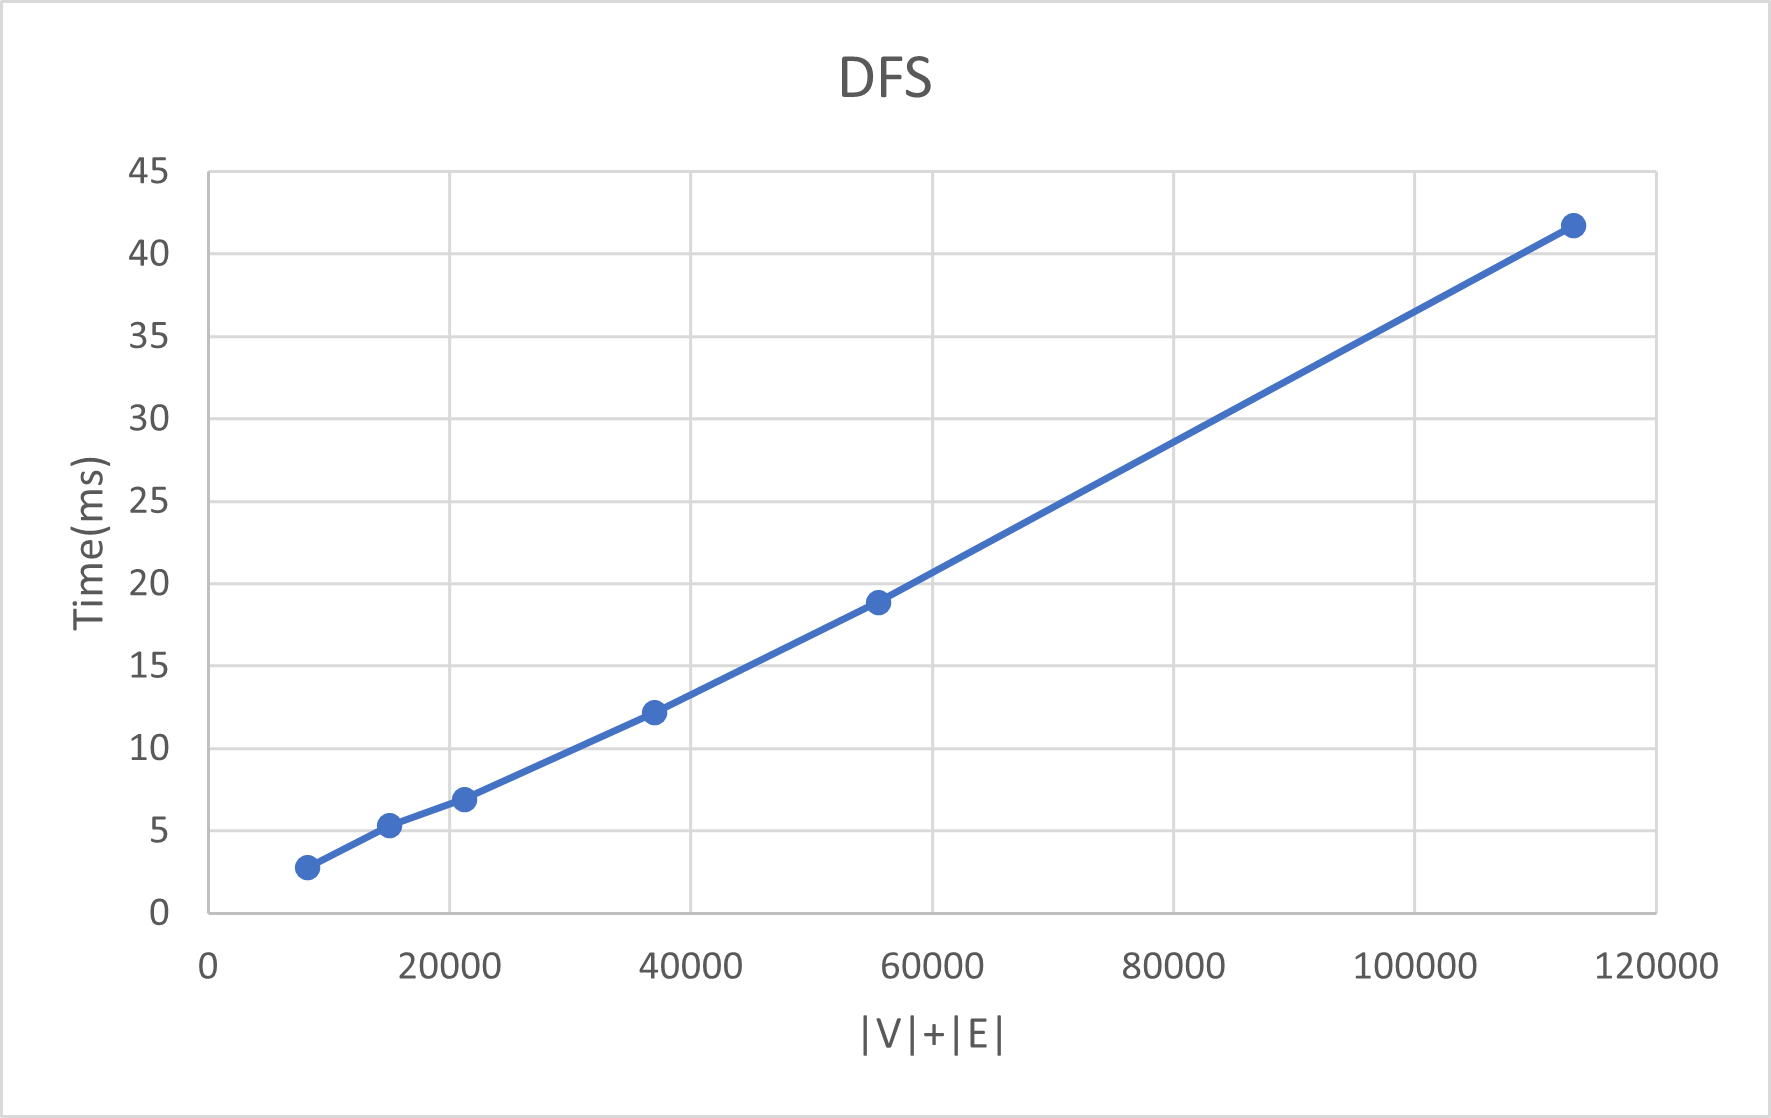
\includegraphics[width=0.6\textwidth]{./imgs/charts/DFSTimeComplexity.png}
	\centering
	\caption{Tempo de execução do algoritmo DFS em ordem a $|V|+|E|$.}
\end{figure}


Como o gráfico indica, obteve-se uma linearidade dos resultados em relação à sua complexidade temporal, pelo que se confirma a complexidade teórica
analisada face aos grafos utilizados.


\section{Breath-First-Search algorithm}
Tal como descrito na secção \hyperref[algo:bfs]{3.1.2}, a complexidade temporal deste algoritmo é da ordem de \( O(|V| + |E|) \).
Para se fazer a análise empírica do algoritmo, foi utilizado o algoritmo quinze vezes em cada mapa (Porto, PortoSCC, Espinho, EspinhoSCC, Penafiel, PenafielSCC).
O gráfico representado de seguida mostra os resultados obtidos em ordem à complexidade temporal teórica:

\begin{figure}[H]
	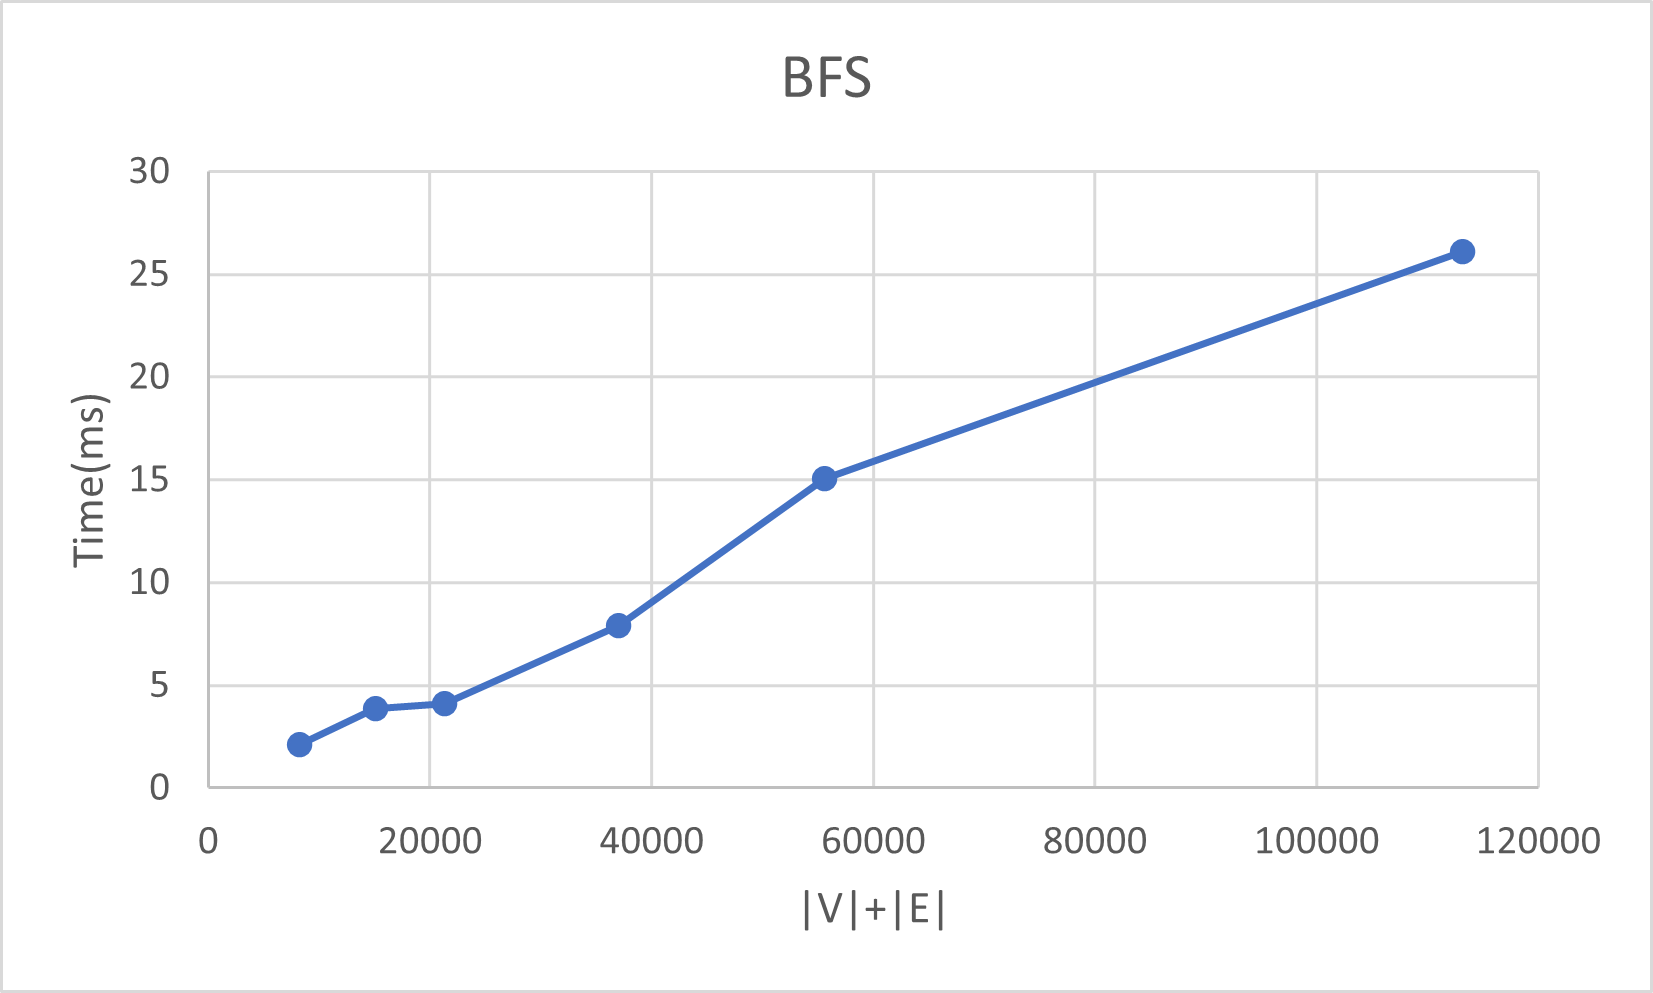
\includegraphics[width=0.6\textwidth]{./imgs/charts/BFSTimeComplexity.png}
	\centering
	\caption{Tempo de execução do algoritmo BFS em ordem a $|V|+|E|$.}
\end{figure}


Como o gráfico indica, obtiveram-se resultados aproximadamente lineares em relação à sua complexidade temporal, pelo que se confirma a complexidade teórica
analisada face aos grafos utilizados.


\section{Kosaraju algorithm}
Tal como descrito na secção \hyperref[algo:kosaraju]{3.2.1}, a complexidade temporal deste algoritmo é da ordem de \( O(|V| + |E|) \).
Para se fazer a análise empírica do algoritmo, foi utilizado o algoritmo quinze vezes em cada mapa (Porto, PortoSCC, Espinho, EspinhoSCC, Penafiel, PenafielSCC).
O gráfico representado de seguida mostra os resultados obtidos em ordem à complexidade temporal teórica:

\begin{figure}[H]
	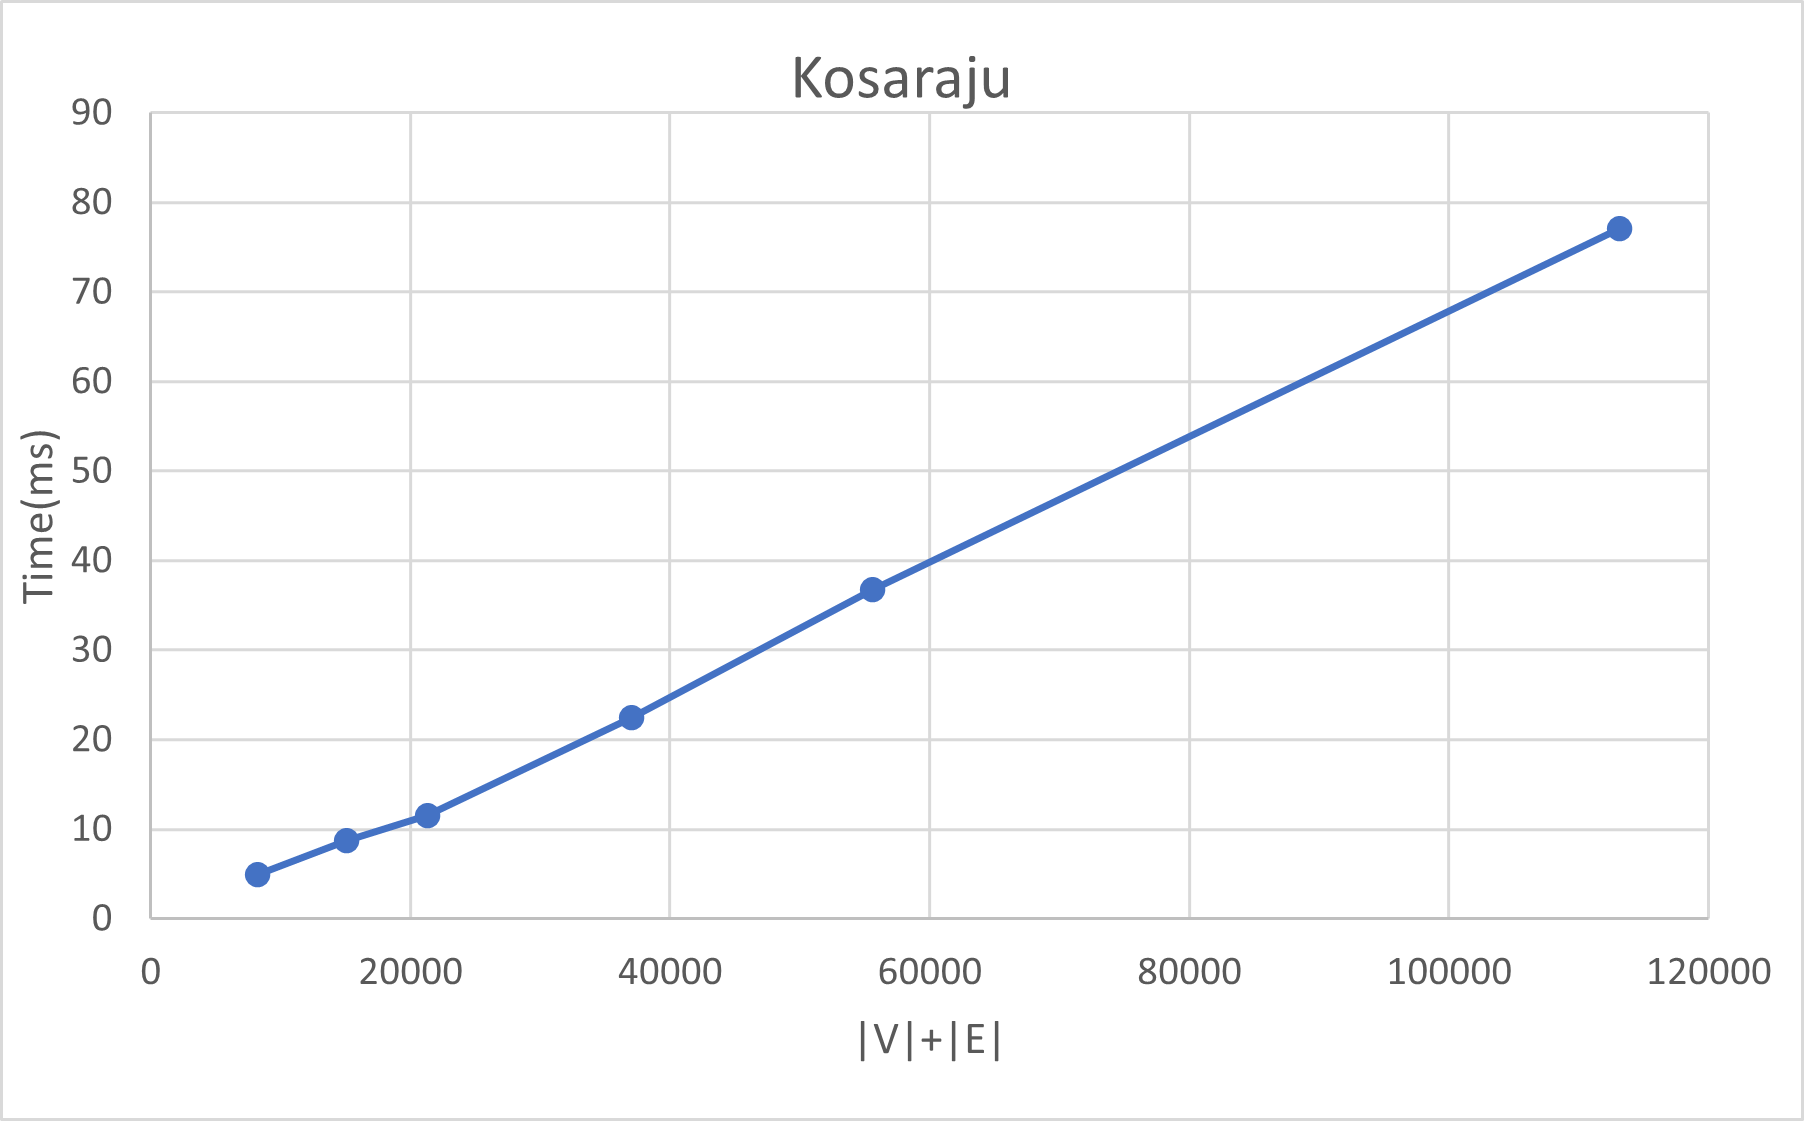
\includegraphics[width=0.6\textwidth]{./imgs/charts/KosarajuTimeComplexity.png}
	\centering
	\caption{Tempo de execução do algoritmo de Kosaraju em ordem a $|V|+|E|$.}
\end{figure}


Como o gráfico indica, obteve-se uma linearidade dos resultados em relação à sua complexidade temporal, pelo que se confirma a complexidade teórica
analisada face aos grafos utilizados.


\section{Dijkstra algorithm}
Tal como descrito na secção \hyperref[algo:dijkstra]{3.3.1}, a complexidade temporal deste algoritmo é da ordem de \( O((|V| + |E|)\cdot \log |V|) \).
Para se fazer a análise empírica do algoritmo, foi utilizado o algoritmo onze vezes em cada mapa (Porto, PortoSCC, Espinho, EspinhoSCC, Penafiel, PenafielSCC).
O gráfico representado de seguida mostra os resultados obtidos em ordem à complexidade temporal teórica:

\begin{figure}[H]
	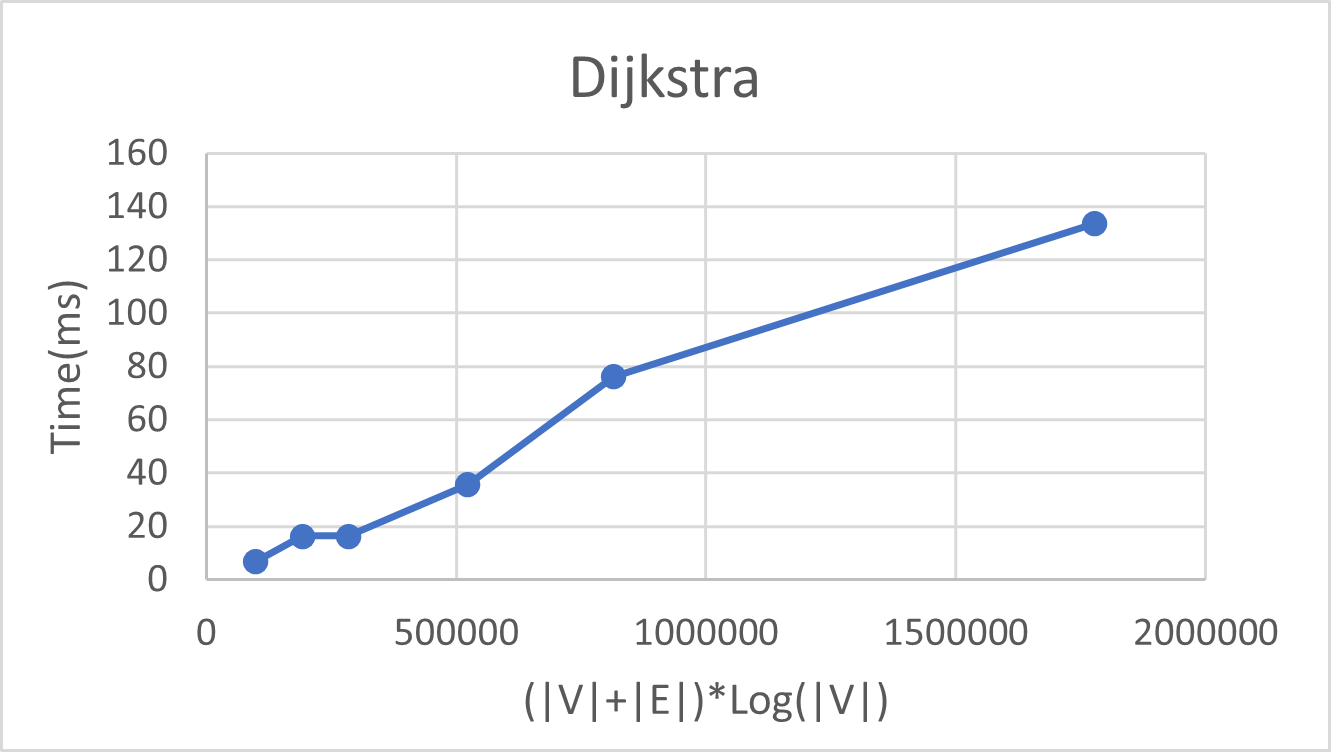
\includegraphics[width=0.6\textwidth]{./imgs/charts/DijkstraTime.png}
	\centering
	\caption{Tempo de execução do algoritmo de Kosaraju em ordem a $(|V|+|E|)\cdot \log |V|$.}
\end{figure}


Como o gráfico indica, obtiveram-se resultados aproximadamente lineares em relação à sua complexidade temporal, pelo que se confirma a complexidade teórica
analisada face aos grafos utilizados.


\section{A* algorithm}
Tal como descrito na secção \hyperref[algo:astar]{3.3.2}, a complexidade temporal deste algoritmo é da ordem de \( O((|V| + |E|)\cdot \log |V|) \).
Para se fazer a análise empírica do algoritmo, foi utilizado o algoritmo onze vezes em cada mapa (Porto, PortoSCC, Espinho, EspinhoSCC, Penafiel, PenafielSCC).
O gráfico representado de seguida mostra os resultados obtidos em ordem à complexidade temporal teórica:

\begin{figure}[H]
	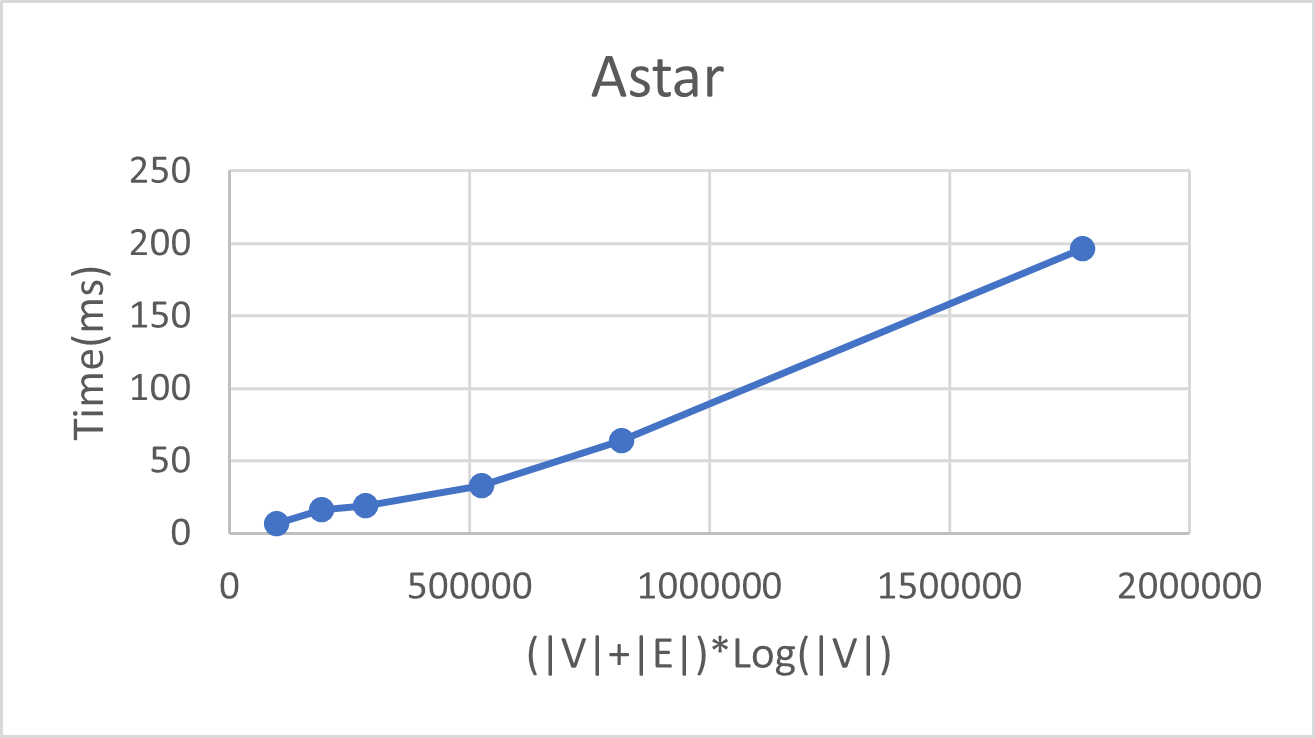
\includegraphics[width=0.6\textwidth]{./imgs/charts/AstarTime.png}
	\centering
	\caption{Tempo de execução do algoritmo A* em ordem a $(|V|+|E|)\cdot \log |V|$.}
\end{figure}


Como o gráfico indica, obteve-se uma linearidade dos resultados em relação à sua complexidade temporal, pelo que se confirma a complexidade teórica
analisada face aos grafos utilizados.


\section{Nearest Neighbor algorithm}
O Algoritmo Nearest Neighbor implementado não tem a complexidade temporal teórica de \( O(|V|^2)\) analisada na secção \hyperref[algo:nn]{3.4.2}, uma vez que foi feita a 
adaptação descrita na seccão \hyperref[implementedAlgos]{Algoritmos efetivamente implementados}. Desta forma, o algoritmo irá percorrer \(|POI|\) vezes o algoritmo de Dijkstra
para obter o ponto de interesse mais próximo não visitado ao ponto de interesse atual. Desta forma, terá uma complexidade da ordem de \( O(|POI| \cdot ((|V| + |E|)\cdot \log |V|)) \).
Para se fazer a análise empírica do algoritmo, foi utilizado o algoritmo onze vezes em cada mapa (Porto, PortoSCC, Espinho, EspinhoSCC, Penafiel, PenafielSCC).
O gráfico representado de seguida mostra os resultados obtidos em ordem à complexidade temporal teórica:

\begin{figure}[H]
	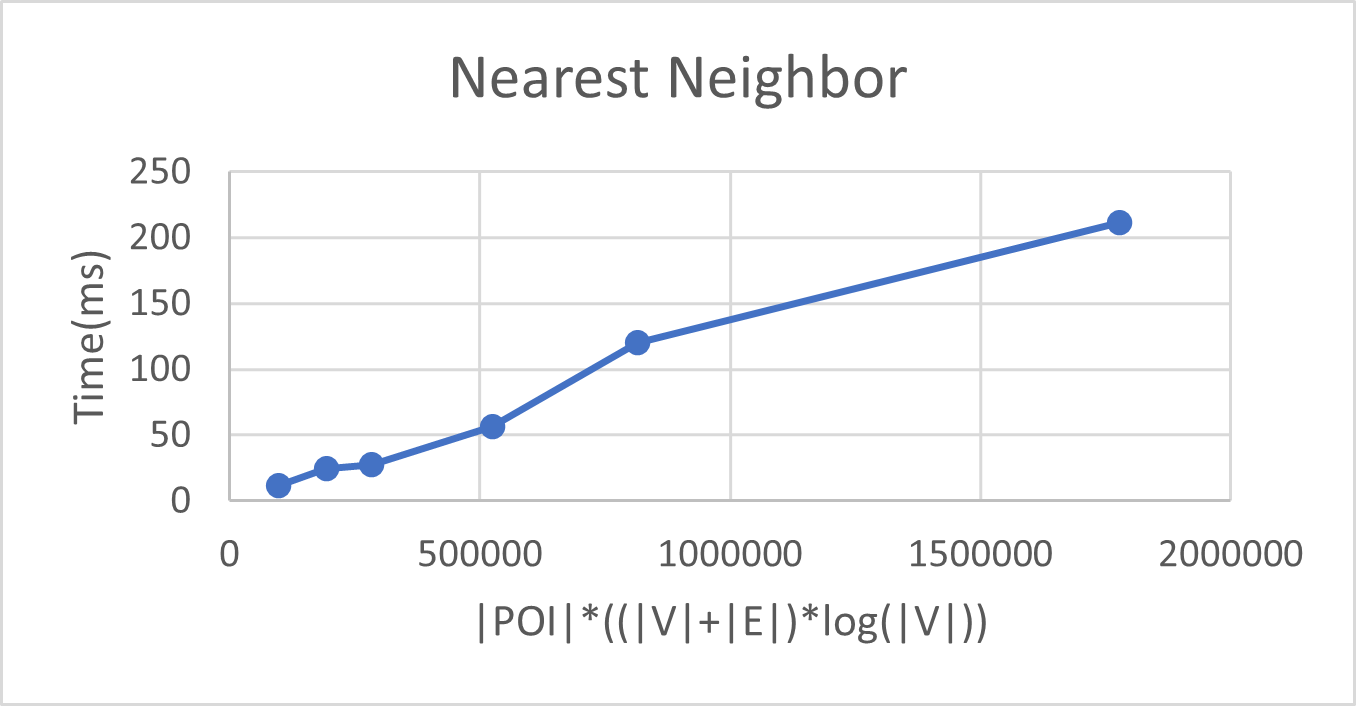
\includegraphics[width=0.6\textwidth]{./imgs/charts/NNTimeComplexity.png}
	\centering
	\caption{Tempo de execução do algoritmo Nearest Neighbor em ordem a $|POI|\cdot (|V|+|E|)\cdot \log |V|$.}
\end{figure}


Como o gráfico indica, obtiveram-se resultados aproximadamente lineares em relação à sua complexidade temporal, 
pelo que se confirma a complexidade teórica analisada face aos grafos utilizados.


\section{Multi-source Dijkstra algorithm}
Tal como descrito na secção \hyperref[algo:msdijkstra]{3.6.1}, a complexidade temporal deste algoritmo é da ordem de \( O((|V| + |E|)\cdot \log |V|) \).
Para se fazer a análise empírica do algoritmo, foi utilizado o algoritmo nove vezes em cada mapa (Porto, PortoSCC, Espinho, EspinhoSCC, Penafiel, PenafielSCC).
O gráfico representado de seguida mostra os resultados obtidos em ordem à complexidade temporal teórica:

\begin{figure}[H]
	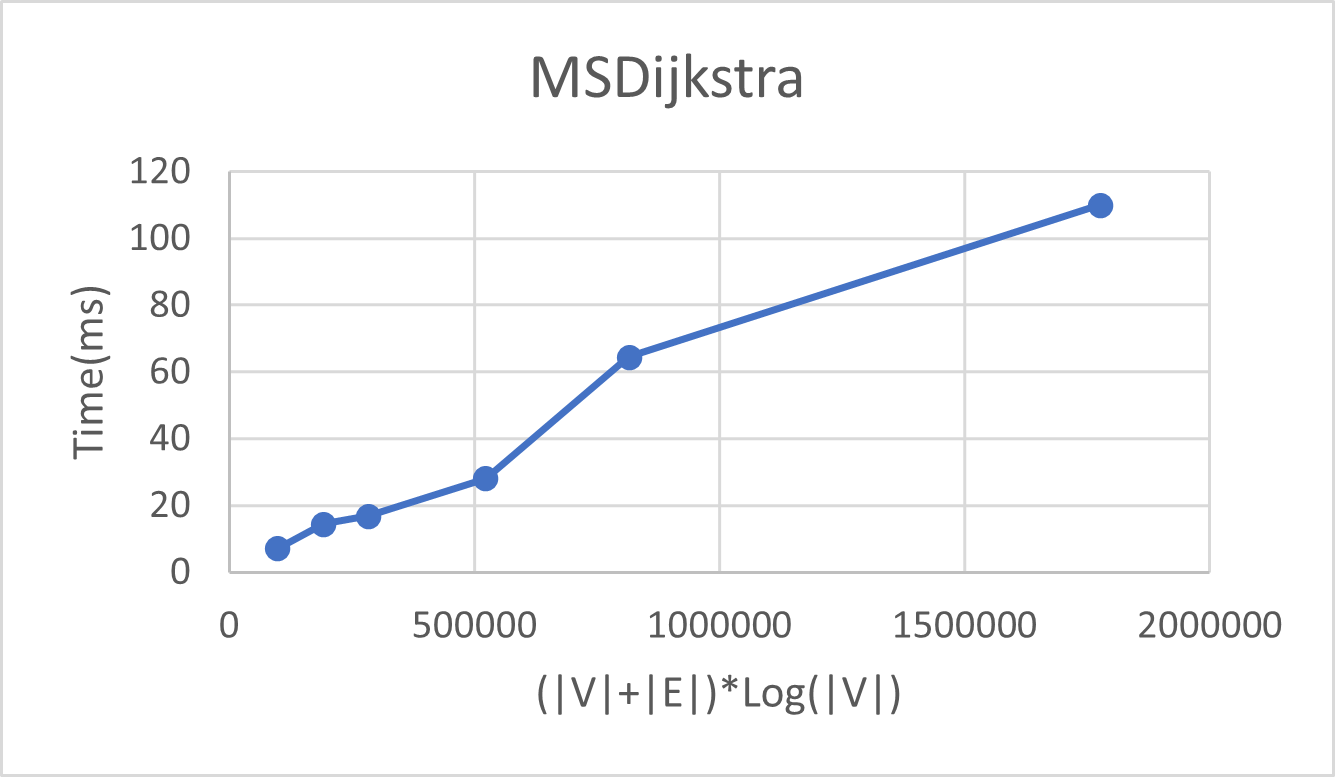
\includegraphics[width=0.6\textwidth]{./imgs/charts/MSDijkstraTimeComplexity.png}
	\centering
	\caption{Tempo de execução do algoritmo Multi-Source Dijkstra em ordem a $ (|V|+|E|)\cdot \log |V|$.}
\end{figure}

Como o gráfico indica, obtiveram-se resultados aproximadamente lineares em relação à sua complexidade temporal, pelo que se confirma a complexidade teórica
analisada face aos grafos utilizados.

\section{Solução do Problema}
De forma a resolver o problema proposto, foram conjugados os algoritmos descritos acima: de modo a verificar se temos caminho de ida e de volta entre
os centros de distribuição e aplicação aplica-se o algoritmo \hyperref[algo:kosaraju]{Kosaraju}, obtendo-se as componentes fortemente conexas; De seguida, fez-se 
a distribuição dos centros de aplicação aos respetivos centros de distribuição, formando-se clusters, com a utilização do algoritmo \hyperref[algo:msdijkstra]{Multi-source Dijkstra};
posteriormente, para se obter o percurso desde os centros de distribuição aos respetivos centros de aplicação onde as carrinhas irão distribuir as vacinas,
utilizou-se o algoritmo \hyperref[algo:nn]{Nearest Neighbor}.
Uma vez que esta implementação final é uma junção, em sequência, de vários algoritmos, a ordem da sua complexidade temporal será igual à ordem da complexidade temporal
do algoritmo com maior complexidade temporal. Assim, a complexidade temporal da implementação será da ordem de \( O(|POI| \cdot ((|V| + |E|)\cdot \log |V|)) \).
Para confirmar esta complexidade, foi utilizado o algoritmo nove vezes em cada mapa (Porto, PortoSCC, Espinho, EspinhoSCC, Penafiel, PenafielSCC).
O gráfico representado de seguida mostra os resultados obtidos em ordem à complexidade temporal teórica esperada:

\begin{figure}[H]
	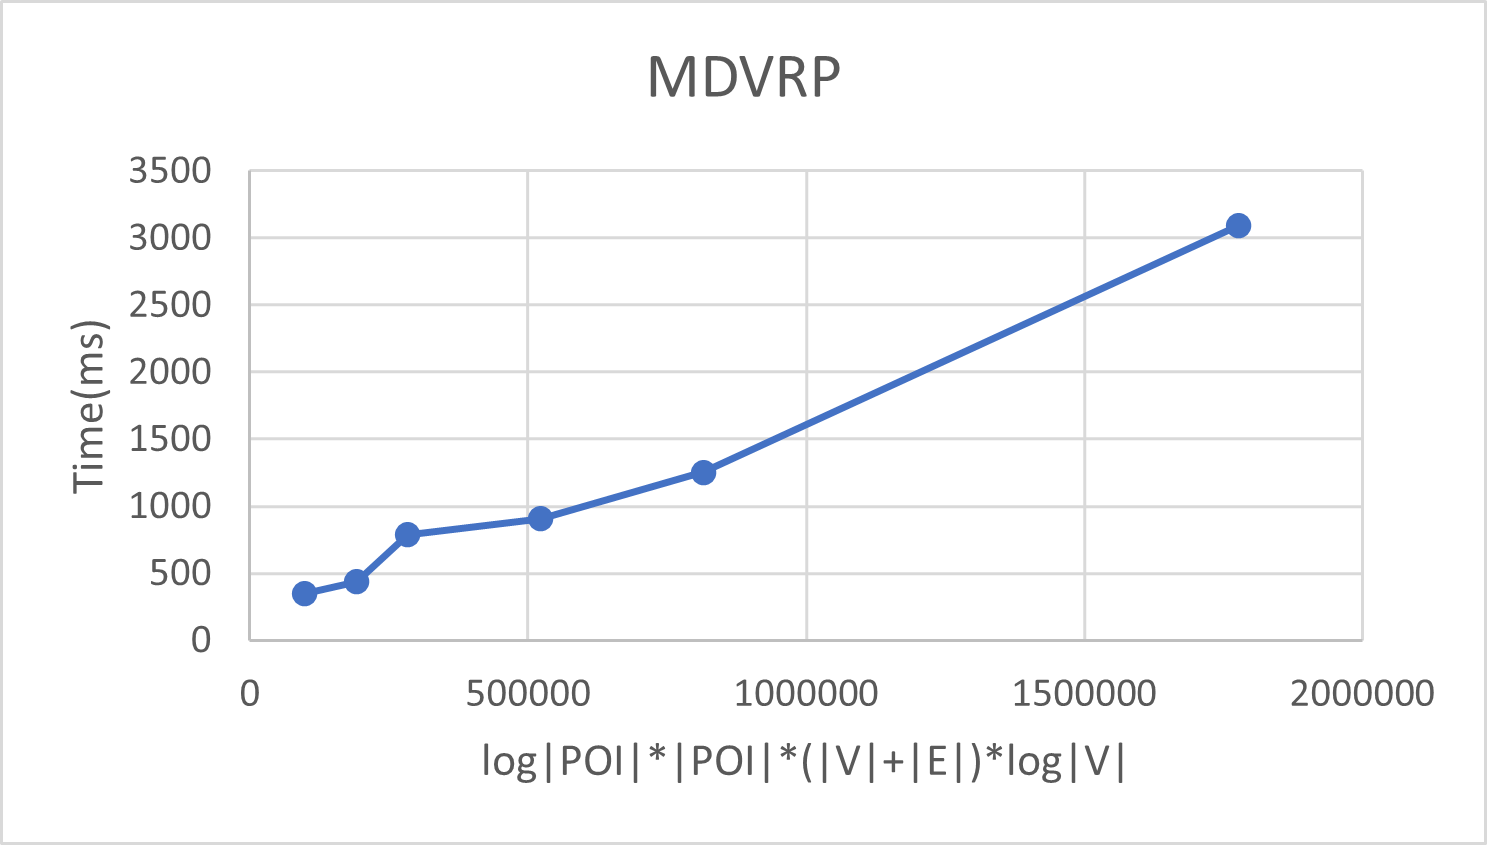
\includegraphics[width=0.6\textwidth]{./imgs/charts/MDVRPTimeComplexity.png}
	\centering
	\caption{Tempo de execução da solução final em ordem a $|POI|\cdot (|V|+|E|)\cdot \log |V|$.}
\end{figure}

Os resultados obtidos foram aproximadamente lineares, pelo que se confirma a complexidade teórica analisada
face aos grafos utilizados.


\chapter{Análise da conectividade do grafo}
De acordo com o a informação dada no problema, pode haver obras na via pública que podem tornar algumas zonas inacessíveis.
Mais do que isto, torna-se ainda necessário que, não só uma carrinha de distribuição consiga chegar aos centro de
aplicação aos quais se pretende levar as vacinas, mas também que tenha caminho de volta. Para este fim, recorreu-se
ao algoritmo de \hyperref[algo:kosaraju]{Kosaraju} que divide o grafo dado em componentes fortemente conexas.
Aplicando isto ao problema em questão, é possível associar a cada centro de distribuição os respetivos Centros 
de aplicação que, devido ao descrito em cima, têm de pertencer à mesma componente conexa. \par

Utilizando a interface do programa, é possível visualizar de forma distinta os vértices pertencentes à
componente fortemente conexa maior dos vértices que pertencem às restantes componentes conexas, sendo estas últimas em grande número
mas cada uma delas com reduzido número de vértices. \par
Nas imagens que se seguem, observam-se as componentes fortemente conexas do Porto, de Espinho e de Penafiel. Como já mencionado 
em \hyperref[func]{Funcionalidades e cenários implementados}, a componente maior é mostrada a amarelo e as restantes a azul, pelo que
nos mapas da componente fortemente conexa os vértices estão todos a amarelo.


\section{Mapa do Porto}

\begin{figure}[H]
	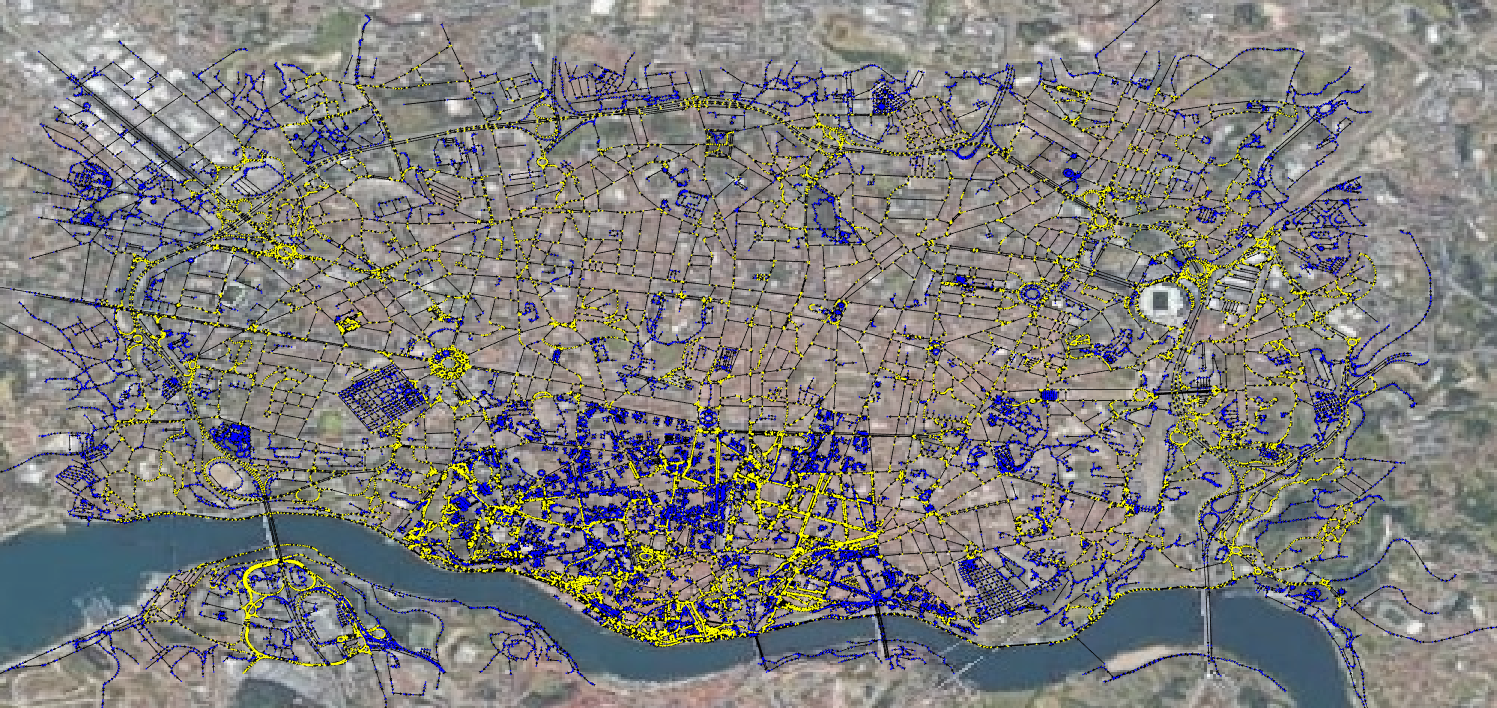
\includegraphics[width=1.0\textwidth]{./imgs/scc/portoSCC.png}
	\centering
	\caption{Componentes fortemente conexas no mapa do Porto completo.}
\end{figure}


\section{Mapa da componente fortemente conexa do Porto}

\begin{figure}[H]
	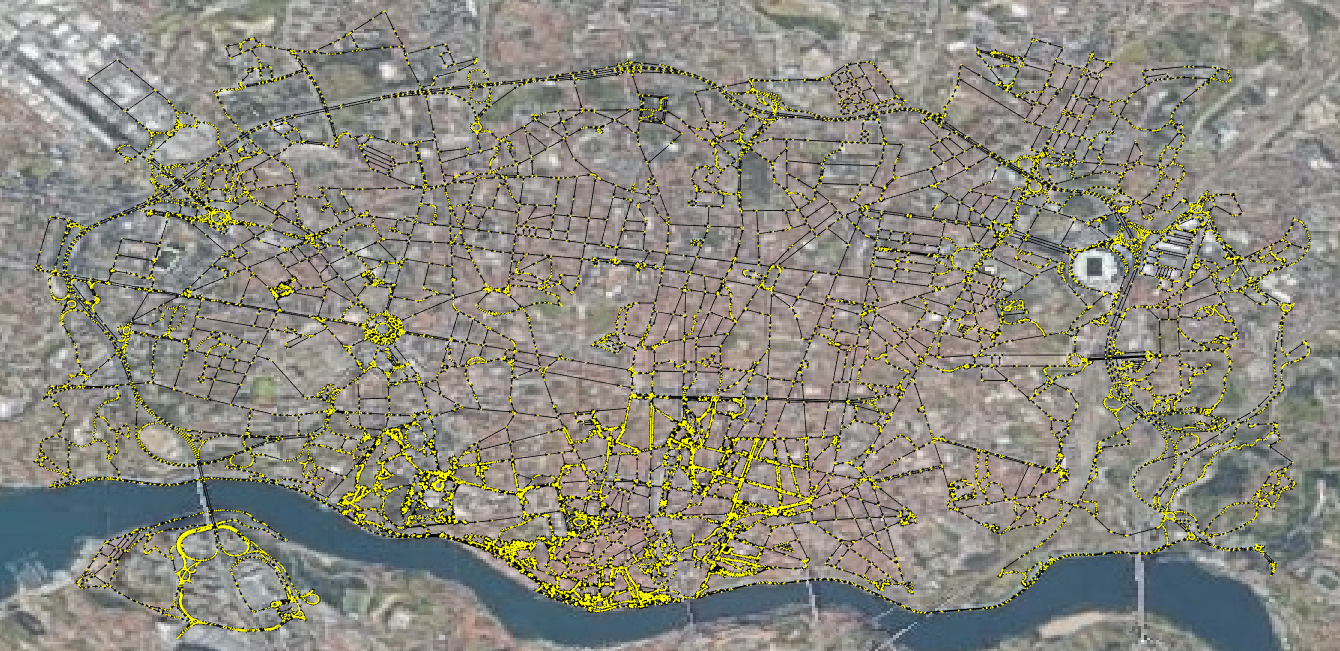
\includegraphics[width=1.0\textwidth]{./imgs/scc/portoStrongSCC.png}
	\centering
	\caption{Componentes fortemente conexas no mapa da maior componente fortemente conexa do Porto.}
\end{figure}


\section{Mapa de Espinho}

\begin{figure}[H]
	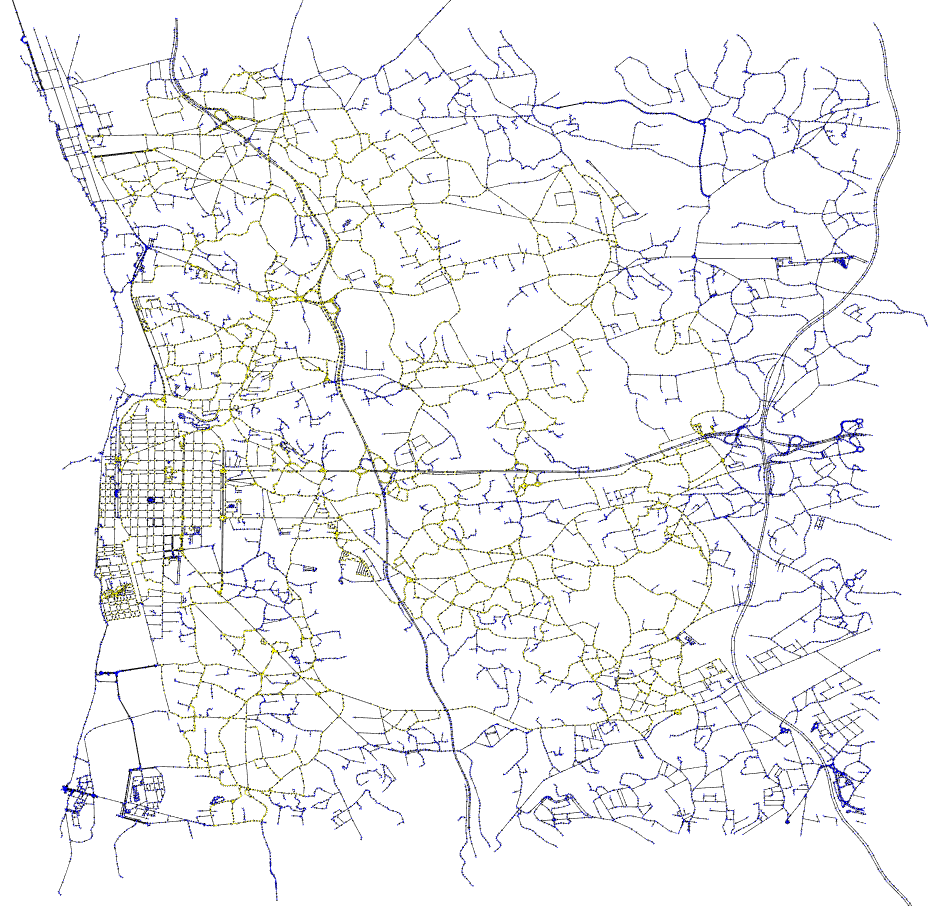
\includegraphics[width=1.0\textwidth]{./imgs/scc/espinhoSCC.png}
	\centering
	\caption{Componentes fortemente conexas no mapa de Espinho completo.}
\end{figure}


\section{Mapa da componente fortemente conexa de Espinho}

\begin{figure}[H]
	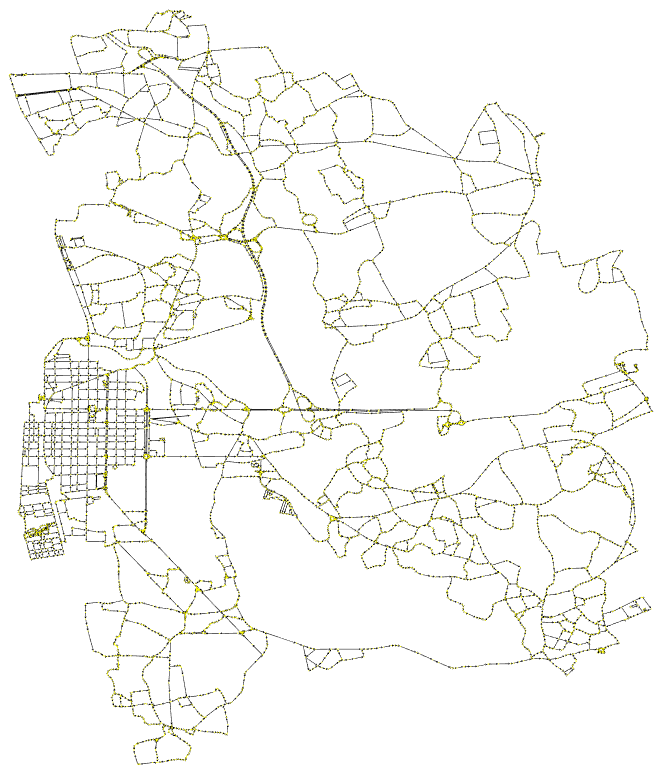
\includegraphics[width=1.0\textwidth]{./imgs/scc/espinhoStrongSCC.png}
	\centering
	\caption{Componentes fortemente conexas no mapa da maior componente fortemente conexa de Espinho.}
\end{figure}


\section{Mapa de Penafiel}

\begin{figure}[H]
	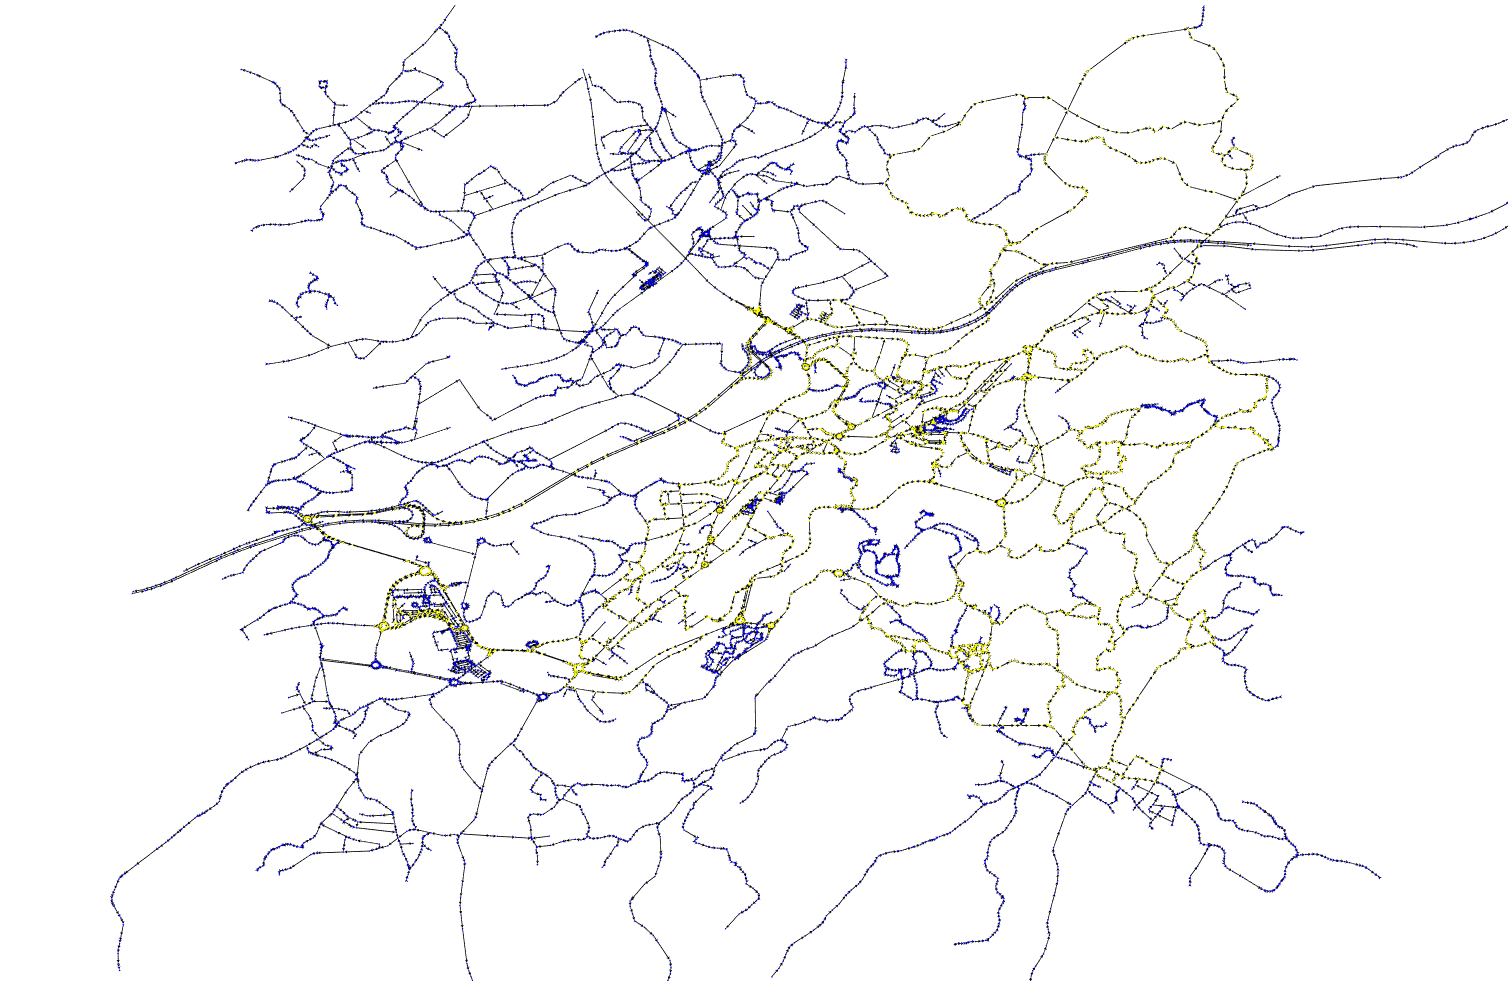
\includegraphics[width=1.0\textwidth]{./imgs/scc/penafielSCC.png}
	\centering
	\caption{Componentes fortemente conexas no mapa de Penafiel completo.}
\end{figure}


\section{Mapa da componente fortemente conexa de Penafiel}

\begin{figure}[H]
	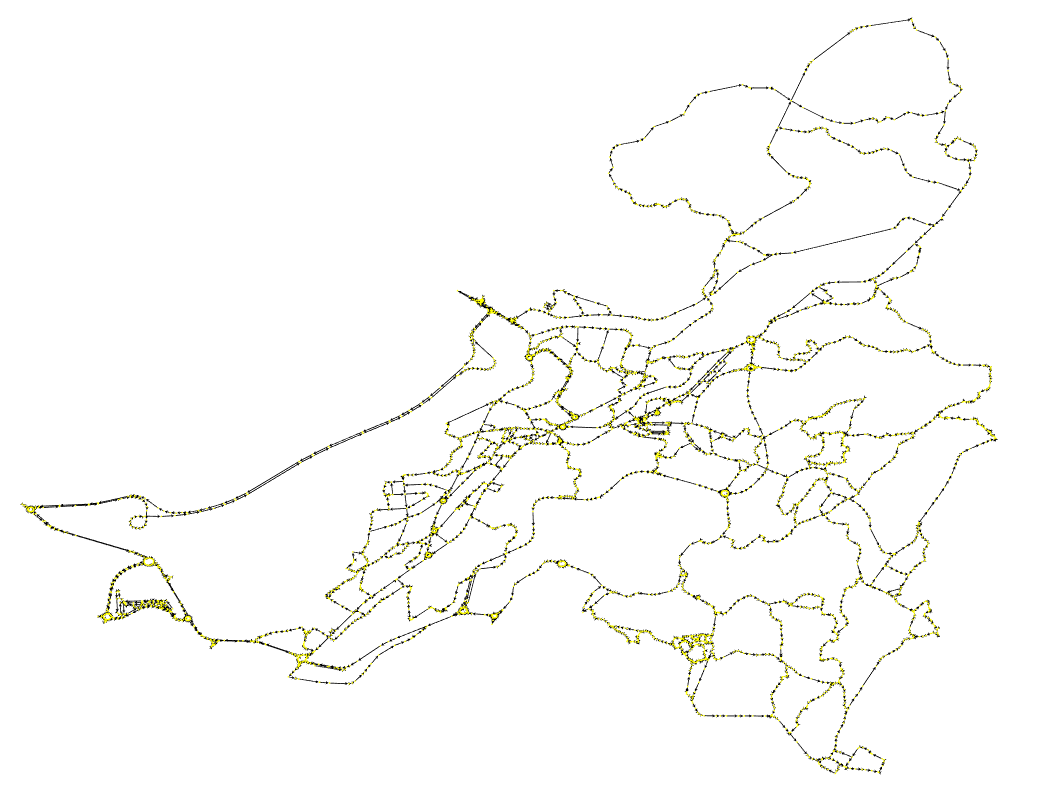
\includegraphics[width=1.0\textwidth]{./imgs/scc/penafielStrongSCC.png}
	\centering
	\caption{Componentes fortemente conexas no mapa da maior componente fortemente conexa de Penafiel.}
\end{figure}



\chapter{Conclusão}

// TODO Mudar esta conclusão
De forma a resolver o problema proposto foram conjugados os algoritmos descritos acima, como se explica de seguida: 
de modo a verificar se temos caminho de ida e de volta entre os centros de distribuição e aplicação aplica-se o algoritmo \hyperref[algo:kosaraju]{Kosaraju}, 
obtendo-se as componentes fortemente conexas; de seguida, faz-se a distribuição dos centros de aplicação pelos centros de distribuição em clusters, utilizando o 
algoritmo \hyperref[algo:msdijkstra]{Multi-source Dijkstra}; posteriormente, para se obter o percurso final, onde as carrinhas saem dos centros de distribuição e distribuem
as vacinas àos respetivos centros de aplicação, utiliza-se o algoritmo \hyperref[algo:nn]{Nearest Neighbor}.


\chapter{Contribuição}
Todos os membros do grupo participaram ativamente na elaboração do trabalho, pelo que a cada um dos três membros é atribuída uma contribuição de \( \frac{100}{3} \% \).


\begin{thebibliography}{9}

	\bibitem{kosaraju}
	Sharir, M. 1981.
	"A strong-connectivity algorithm and its application in data flow analysis."
	\textit{Computers \& Mathematics with Applications} 67-72.

	\bibitem{tarjan}
	Tarjan, R. E. 1972.
	"Depth-first search and linear graph algorithms."
	\textit{SIAM Journal on Computing} 146-160.

	\bibitem{astar} 
	Hart, Peter E., Nils J. Nilsson, and Bertrand Raphael. 1968. 
	"A Formal Basis for the Heuristic determination of Minimum Cost Paths." 
	\textit{IEEE Transactions on Systems Science and Cybernetics} 4 (2): 100-107.

	\bibitem{bellmanheldkarp}
	Spoerhase, Joachim, Thomas van Dijk, and Alexander Wolff. 2019/20.
	"Lecture 1. Introduction \& Held-Karp-algorithm for TSP."
	\textit{Slides for Advanced Algorithms course in Universität Würzburg}, 39-55.
	
	\bibitem{nearestneighbor} 
	Chanzy, P. 1993
	"Range Search and Nearest Neighbor Search."
	\textit{Master’s Thesis, McGill University.}

	\bibitem{cormen}
	Cormen, Thomas H., Charles E. Leiserson, Ronald L. Rivest, e Clifford Stein. 2009.
	\textit{Introduction to Algorithms}. 3rd. MIT Press.

	\bibitem{weiss}
	Weiss, Mark Allen. 2013.
	\textit{Data Structures and Algorithm analysis in C++}. 4th. Pearson.

	\bibitem{slidesCAL}
	Rossetti, R., A. P. Rocha, L. Ferreira, J. P. Fernandes, F. Ramos, G. Leão. 2021
	\textit{Slides for Concepção e Análise de Algoritmos course in FEUP, MIEIC}.

\end{thebibliography}


\end{document}
